\documentclass[a4paper,twoside,12pt,titlepage,openright]{book}

\frontmatter
\pagenumbering{Roman}

\usepackage{tabularx}
\usepackage{booktabs}                                  % to write algorithms
\usepackage{verbatim}                                         % to comment
\usepackage{rotating}                  % rotates the figures to landscape
\usepackage{anyfontsize}
\usepackage{subfig}
\usepackage{amsmath}
\usepackage{mwe}
\usepackage{siunitx}
\sisetup{
	range-phrase = {,},
	range-units  = brackets
}
\usepackage{amsthm}
\usepackage{epstopdf}
\usepackage{amsfonts}    
\usepackage{gensymb}                                     % for the letters of the sets
\usepackage{graphicx}                                          % to insert images
\usepackage[export]{adjustbox}
\usepackage{xcolor}
\usepackage[italian, english]{babel}							%language
\usepackage[utf8]{inputenc}
\usepackage[T1]{fontenc}
\usepackage[dvips]{epsfig}
\usepackage{bm}                                                  % bold formulas 
\usepackage{fancyhdr}
\usepackage{amsmath}
\usepackage{amssymb}
\usepackage{a4}
\usepackage{frontespizio}
\usepackage{hyperref}
%\usepackage{float}
\usepackage{appendix}
\usepackage[nopostdot, nonumberlist, acronym]{glossaries}
\usepackage[autostyle]{csquotes}
\usepackage{floatrow}
\usepackage{subfig}
\usepackage[a4paper,twoside, inner =25mm, outer =25mm, top =30mm, bottom =30mm, bindingoffset =10mm,nomarginpar]{geometry}
\setcounter{secnumdepth}{3}
\setcounter{tocdepth}{3}
\usepackage{algorithm}
\usepackage{algpseudocode}
\algnewcommand\algorithmicforeach{\textbf{for each}}
\algdef{S}[FOR]{ForEach}[1]{\algorithmicforeach\ #1\ \algorithmicdo}
\usepackage{kpfonts}
\usepackage{stackengine,scalerel}
\usepackage{calc}
\usepackage[square, numbers, sort&compress]{natbib}
\usepackage{multirow}
\bibliographystyle{abbrvnat}
\newlength\shlength
\newcommand\longvec[2][0]{\ThisStyle{\setlength\shlength{#1\LMpt}%
		\stackengine{-5.6\LMpt}{$\SavedStyle#2$}{\smash{$\kern\shlength%
				\stackengine{\dimexpr 1.3pt+6.25\LMpt}{$\SavedStyle\mathchar"017E$}%
				{\rule{\widthof{$\SavedStyle#2$}}{\dimexpr.1pt+.5\LMpt}\kern.4\LMpt}{O}{r}{F}{F}{L}\kern-\shlength$}}%
		{O}{c}{F}{T}{S}}}
\newcommand{\pushcode}[1][1]{\hskip\dimexpr#1\algorithmicindent\relax}

\hypersetup{
	colorlinks   = true, %Colours links instead of ugly boxes
	urlcolor     = black, %Colour for external hyperlinks
	linkcolor    = black, %Colour of internal links
	citecolor   = black %Colour of citations
}

\DeclareMathOperator{\sgn}{sgn}
\graphicspath{{./Images/}}

\theoremstyle{plain}
\newtheorem{teorema}{Teorema}
\theoremstyle{definition}
\newtheorem{definizione}{Definizione}
\graphicspath{{Images/}}
\DeclareGraphicsExtensions{.ps,.eps}
\linespread{1.5}
\setlength{\headheight}{15pt}
\emergencystretch=2em

% For theorems and definitions
\theoremstyle{definition}
\newtheorem{definition}{Definition}[chapter]
\theoremstyle{plain}
\newtheorem{theorem}{Theorem}[chapter]

\setlength{\parskip}{\baselineskip}
\setlength{\parindent}{0pt}







\begin{document}

\begin{titlepage} %inizio frontespizio
    \begin{center} %centra quanto scritto sotto
    \LARGE \textbf{POLITECNICO DI MILANO}\\
    \vspace{0.1cm} %metti uno spazio verticale di 0.1 cm
    
    
    \large School of Industrial and Information Engineering\\Master of Science in Automation and Control Engineering
    \vspace{1cm}
    
    \begin{figure}[!h]\centering
\includegraphics[width=7cm]{logo_new.png}\end{figure}
    \vspace{.8cm}
    
    {\LARGE \textbf{Pose Estimation and Semantic Meaning Extraction for Robotics Using Neural Networks}} %thesis title
    
    \end{center} %fine centra
    \vspace{1.2cm}
    
    \begin{flushleft}
        \begin{tabbing}
            \large{Supervisor: \hspace{1.25cm}}\=\large{Prof. Paolo Rocco}\\
            \large{Co-supervisors: \hspace{0.3cm}}\=\large{Prof. Andrea Maria Zanchettin}\\
            \large{\hspace{4cm}}\=\large{Ing. Niccolo Lucci}\\
        \end{tabbing}
    \end{flushleft}
    
    \vspace{0.5cm}
    
    \large \begin{flushright} %metti a destra
        Master Thesis dissertation of:
    \end{flushright}
    \vspace{-0.9cm}
    \large
    \begin{flushright} 
        Davide Figundio\\
        Id: 965898\\
        Academic year 2022-2023
    \end{flushright}
    
\end{titlepage} %fine frontespizio

\afterpage{\null\newpage}

\pagestyle{empty}
\vspace{17cm}

%\large
\begin{flushright}
\itshape{Scrivi qui la tua dedica}
\end{flushright}






    


\thispagestyle{empty}  

\begin{otherlanguage}{italian}
\chapter*{Ringraziamenti} 
\markboth{}{}
%\addcontentsline{toc}{chapter}{Ringraziamenti} 
Ringrazio  ....\\
Un ulteriore ringraziamento è rivolto a...
\end{otherlanguage}
	

\pagestyle{fancy}
\renewcommand{\chaptermark}[1]{\markboth{#1}{}}
\renewcommand{\sectionmark}[1]{\markright{\thesection\ #1}}
\fancyhf{} \fancyhead[LE,RO]{\bfseries\thepage}
\fancyhead[LO]{\bfseries\rightmark}
\fancyhead[RE]{\bfseries\leftmark}
\renewcommand{\headrulewidth}{0.5pt}
\renewcommand{\footrulewidth}{0pt}
\fancypagestyle{plain}{
\fancyhead{}
\renewcommand{\headrulewidth}{0pt}}

%%%%%%%%%%%%%%%%%%%%%%%%%%%%%%%%%%%%%%%%%%%%%%%%%%%%%%%%%%%
\tableofcontents
%%%%%%%%%%%%%%%%%%%%%%%%%%%%%%%%%%%%%%%%%%%%%%%%%%%%%%%%%%%

\mainmatter

\chapter*{Abstract} 
\markboth{Abstract}{Abstract}
\addcontentsline{toc}{chapter}{Abstract}
With the introduction of Convolutional Neural Networks, the fields of object detection and 6D pose estimation from RGB images have seen large advancements in accuracy and technique. We investigate to verify the applicability of these black-box methods for perception tasks in the fields of industrial and collaborative robotics. In particular we devise a method for generating realistic training datasets for objects in a predetermined environment starting from photographs, greatly facilitating the usually laborious and expensive data acquisition phase that is considered to be a pre-requisite for machine learning applications. We then trained a neural network on various experimental datasets of this sort to evaluate its performance. We also devised an approach te extrapolate the semantic state of a scene from the ouputs of a pose estimation network. Finally, we demonstrated the performance of our methods in a real-world scenario by using the output of a trained neural network to plan the movement of a robotic manipulator. 

\textbf{Keywords:} Robotics, Machine Learning, AI, Neural Networks, Semantics, Pose Estimation.
\label{ch:state_of_the_art}

In this chapter we will give an overview of 6D pose estimation methods. Pose estimation is subject to ongoing research, as it has wide applicability in a variety of fields, including but not limited to robotics, autonomous vehicles, augmented reality and computer vision.

\section{Non-Learning-Based Methods}
\label{s:notlearningbasedmethods}

Before deep learning became widespread, other methods existed for determining a 6D pose from an image. 

The first pose estimation algorithms worked through image segmentation and voting schemes. In 1972, Dula and Hart started using Hough\cite{Hough} voting to detect lines and curves in images\cite{HoughLines}, and Ballard later generalised this procedure to analytically defined shapes\cite{generalisedHough}, popularizing its application for computer vision. In parallel, Lamdan and Wolfson published their Geometric Hashing\cite{GHashing} method, which is based on the representation and matching of objects using their minimal features, such as points or lines.

More modern approaches can be divided into three sub-categories. 2D-3D correspondence methods aim to recognize features in an image and match them to known object characteristics \cite{SURF}, but often rely on texture information, and cannot be applied to textureless objects. Real-image-based methods\cite{ImageMatching} transform the pose estimation problem into an image-matching problem, associating the detected image to a database of previously saved templates. This requires a difficult and time consuming process to acquire these reference images. CAD image-based methods\cite{CADMatching} aim to circumvent this by rendering the references using a 3D model. All of these approaches have issues with adapting to new situations, such as strong changes in illumination, cluttered scenes, and repeated objects.

A very easy way to identify the 6D pose is through the use of markers. When placed on an object and photographed, these markers highlight the points on the image that correspond to the 3D location of the marker, and the pose can then be obtained by solving a Perpective-n-Points\cite{PnP} (PnP) problem. For example, an ArUco marker\cite{Aruco}, can be easily and robustly detected by applying image thresholding and contour extraction, and its pose estimated by using its corners as keypoints\cite{ArucoDetection}. The obvious downside of this method is that it requires markers to be applied to objects, which is often not feasible. A second downside is that it also does not perform in case of partial or total occlusions of the marker(s).

Overall, non-learning based methods, while simple and computationally efficient, often require strictly controlled enviroments and specific conditions to be functional. This greatly restricts their applicability, and therefore learning-based methods are more widely used.

\section{Learning-Based Methods}
\label{s:learningbasedmethods}

Since the introduction of Convolutional Neural Networks (CNN), artifical intelligence and deep learning have been widely applied to the field of image processing, including its subfields of object detection and 6D pose estimation. The methods described in this section aim to train a CNN on vast quantities of data to perform a certain task. Based on the specifics of this task, we can categorize these approaches into three main branches: 2D-3D correspondence, direct estimation, and pose refinement. We will give a couple of examples for each of these categories.

\subsection{2D-3D Correspondence}
\label{ss:2D3D}

This class of methods uses a two step approach: they first implement a neural network to regress a set of 2-D points from an image, corresponding to a set of known feature points, and then use PnP to obtain the 6D pose of the object.

BB8\cite{BB8} uses object segmentation to perform 2D object detection, then regresses the 8 points that form the 3D bounding box of an object, but struggles with textureless symmetric or partially occluded objects. To combat these issues, PVNet\cite{PVNet} uses farthest point sampling to select keypoints on the surface of the object, and then implements a dense pixel-wise voting network, where each pixel "votes" on locations for the keypoints. RANSAC\cite{RANSAC} is then used to exclude outliers and obtain predictions with their probability distribution, which are then used for uncertainty-driven PnP.

Most approaches in this class share two common weaknesses. First, they are very perfomance-intensive when estimating the pose of multiple objects, since keypoint regression and PnP have to be computed for each object individually\cite{bukschat2020efficientpose}. Second, they are not end-to-end trainable, as the loss functions implemented do not reflect the final perfomance on the pose estimation task\cite{SS6D}. However, recent approaches have faced this issue by implementing learned or differentiable PnP algorithms, so as to enable end-to-end training\cite{EPro-Pnp}.

\subsection{Direct Estimation}
\label{ss:directestimation}

The approaches in this category use convolutional neural networks to directly regress the pose of an object in a single step. They are end-to-end trainable and boast better run times than the previously seen 2D-3D methods.

PoseNet\cite{PoseNet} was one of the first implementations of this concept, and was originally conceptualized for obtaining the camera pose from outdoor or indoor enviroments, and not for object pose estimation. Deep-6DPose\cite{deep6D} works by extending the Mask R-CNN\cite{Mask-R-CNN} instance segmentator, which in turn extends the Faster R-CNN\cite{Faster-R-CNN} object detector, and introduced a key technical feature by decoupling rotation and translation parameters, so as to make the pose regression loss differential. PoseCNN\cite{PoseCNN} expanded on this idea, and introduced a novel loss function that enabled it to properly handle symmetric objects.

Most networks in this category are fast and relatively accurate, but struggle in situations with partial occlusions.

\begin{table}[ht]
    \begin{center}
        \begin{tabular}{||c c c c c||} 
        \hline
        Rank & Model Name & Mean ADD & Method & Year\\ [0.5ex] 
        \hline\hline
        1 & RNNPose & 97.37 & Refinement & 2022 \\ 
        \hline
        2 & EfficientPose & 97.35 & Direct Estimation + Refinement & 2020 \\
        \hline
        3 & RePOSE & 96.1 & Refinement & 2021 \\
        \hline
        4 & EPro-PnP-6DoF v1 & 95.8 & 2D-3D & 2022\\
        \hline
        5 & ROPE & 95.61 & 2D-3D & 2021 \\
        \hline
        6 & DPOD & 95.2 & 2D-3D + Refinement & 2019\\
        \hline
        7 & HRNet  & 93.3 & 2D-3D & 2019 \\
        \hline
        8 & HybridPose & 91.3 & 2D-3D & 2020 \\
        \hline
        9 & CDPN & 89.86 & 2D-3D + Direct Estimation & 2019 \\
        \hline
        10 & PoseCNN + DeepIM & 88.6 & Direct Estimation + Refinement & 2018\\
        \hline
        \end{tabular}
    \caption{Top ten performing models on the LINEMOD dataset\cite{linemod} as of November 2022. Data taken from paperswithcode.com/sota/6d-pose-estimation-on-linemod.}
    \label{tab:top10models}
    \end{center}
\end{table}

\subsection{Pose Refinement}
\label{ss:poserefinement}

Approaches in this category rely on an inital estimate of the 6D pose, and then use various methods to refine it so as to obtain a more precise prediction.

DeepIM\cite{DeepIM} employs an iterative approach, by repeatedly rendering a 3D model of the object and matching it against the observed image. To ensure successive iteraterations gain in precision, it is trained not only on an annotated dataset, but also on previous outputs of the network. RNNPose\cite{RNNPose}, while also starting from a rendering and the observed image, formulates the task as a nonlinear optimization problem: it minimizes differences between correspondence fields by leveraging recent discoveries in the field of optical flow estimation, while recurrently calling itself. RNNPose currently boasts the best performance on the widely used LINEMOD\cite{linemod} dataset.

While refinement methods achieve remarkable performance, they have two main downsides. First, they rely on an inital estimate of the pose, so they cannot be applied independently, and second, they are relatively computationally intensive, especially when one considers that they must be run in parallel with another estimation method to generate the initial poses.

\begin{figure}[h]
    \centering
    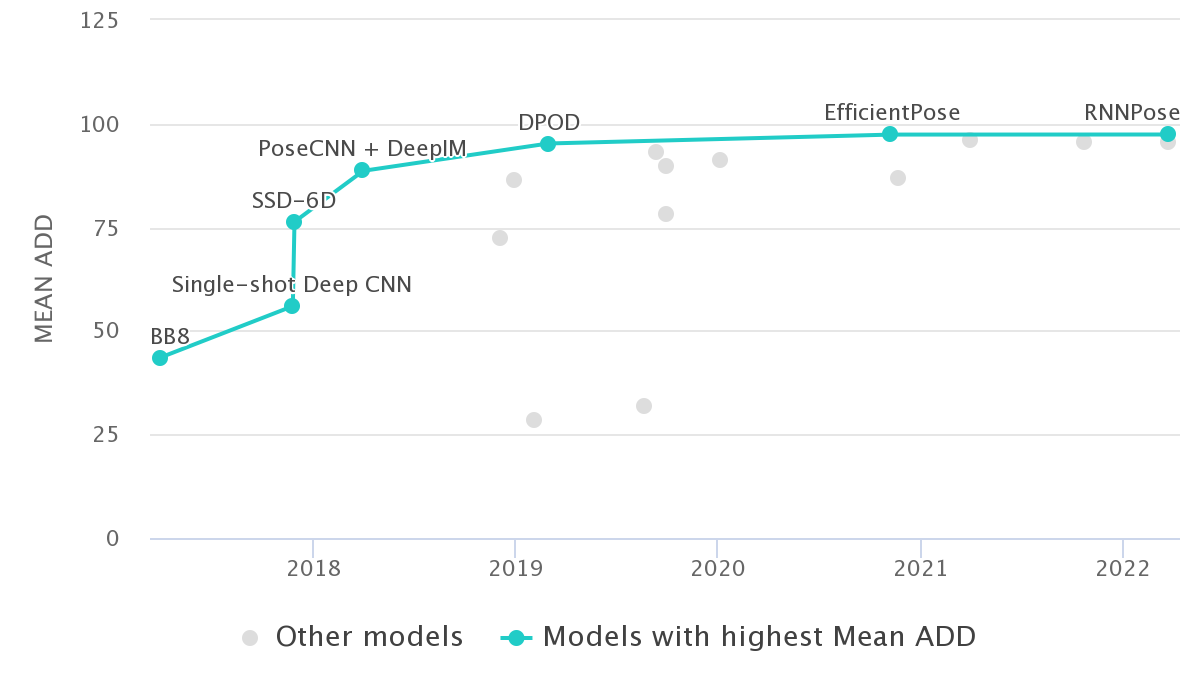
\includegraphics[width=0.7\textwidth]{linemodchart.png}
    \caption{Performance on LINEMOD of recent pose estimation algorithms by year. Graphic originates from paperswithcode.com/sota/6d-pose-estimation-on-linemod.}
    \label{fig:linemodchart}
\end{figure}

\subsection{Conclusions on Learning Approaches}

Data-driven models based on deep learning are generally considered superior to non-learning-based models. A wide variety of approaches exists, and each approach brings its own distinct advantages. When choosing a model, special attention must be given to the requirements for the application the model is destined for. Overall, recent approaches have been dominated by variations on 2D-3D correspondence and refinement methods, with a few exceptions.

\section{EfficientPose}

EfficientPose was chosen as the starting point for this thesis as it boasts state-of-the-art results while maintaining relative simplicity and low computational cost. It was designed with multi-object estimation in mind, which is especially significant, as other approaches do not scale well with the number of total detections.

Similarly to Deep-6DPose (previously mentioned in section \ref*{ss:directestimation}), it is an end-to-end direct 6D pose estimation approach that extends the functionality of a 2D network. While Deep-6D extends the segmentation network Mask-R-CNN, EfficientPose extends Google's object classification network EfficientDet\cite{EfficientDet}, which in turn builds on Google's backbone network EfficientNet\cite{EfficientNet}. We will briefly examine these two network families.

We specify "families," as both networks are based on the concept of scalability. They provide a baseline network, and then scale up its depth, width and resolution using a single hyperparameter ($\phi$) to achieve better performance when necessary. EfficientNet is designed using neural architecture search\cite{NAS} to provide optimal structure for the baseline, while EfficientDet expands upon this backbone by introducing a feature pyramid network\cite{FPN} (FPN).

FPNs are built for multi scale feature fusion, combining information contained in low resolution, semantically strong features with information containted in high resolution, semantically weak features. EfficientDet implements its own version of FPN, called bi-directional FPN, where top-down and bottom-up aggregation paths are then repeated a number of times dependant on the chosen $\phi$. The outputs of the Bi-FPN are then fed into two fully connected networks that perform class and bounding box prediction.

\begin{figure}[h]
    \centering
    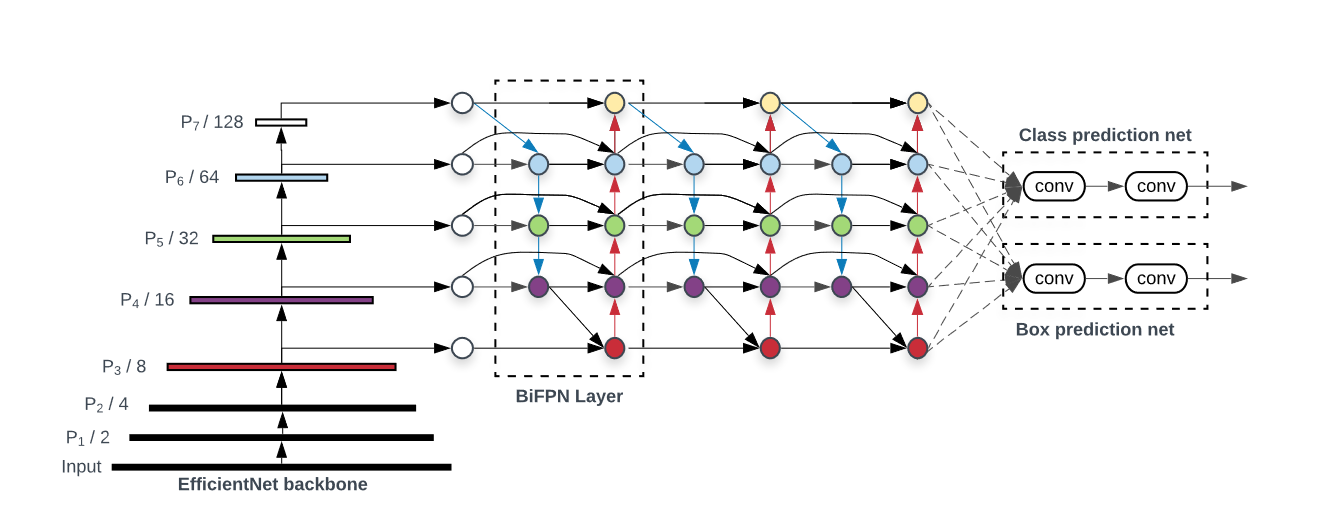
\includegraphics[width=0.9\textwidth]{EfficientDetArchitecture.png}
    \caption{Overview of the EfficientDet architecture. BiFPN layers and Class/Box layers may be repeated multiple times according to resource constraints.}
\end{figure}

\begin{figure}[ht]
    \centering
    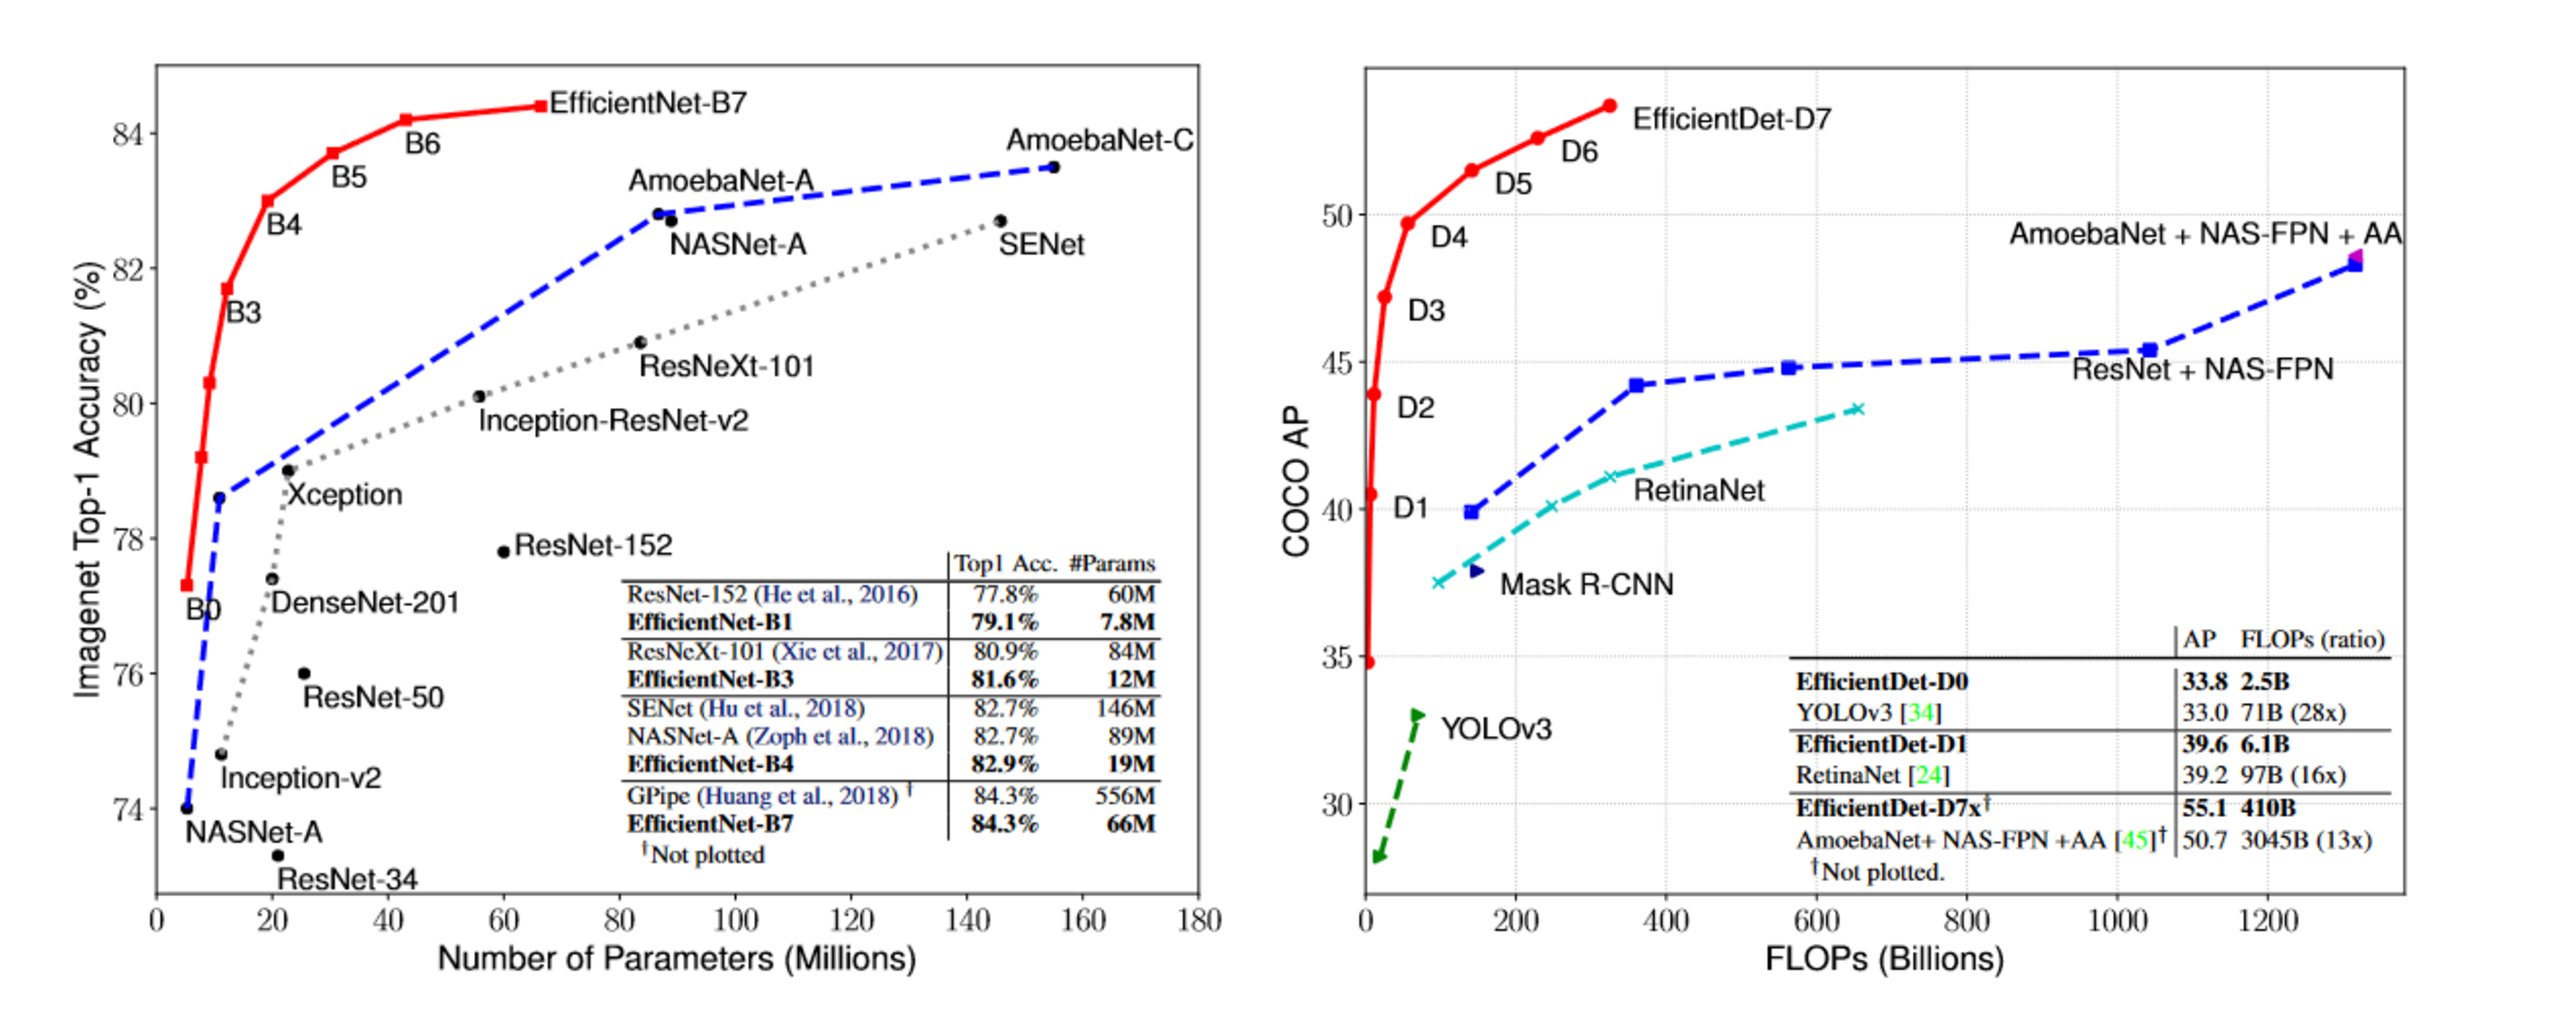
\includegraphics[width=\textwidth]{EfficientDetNetPerfromance.png}
    \caption{Performance of EfficientNet and EfficientDet relative to other approaches for various values of $\phi$. EffcientNet is evaluated on the ImageNet database\cite{imagenet}, while EfficientDet is evaluated on the Microsoft Common Objects in Context database\cite{cocodataset}. Images are taken from the relative papers on EfficientNet and EfficientDet.}
\end{figure}

The resulting network has the characteristic of being a single-shot object detector. This sets it apart from previously mentioned approaches such as Mask-R-CNN, which employ a two phase approach, with an initial region proposal step followed by the final object detection. By applying a single step approach, EfficientDet is much simpler and computationally efficient.



EfficientPose's expansion on this architecture is extremely simple, adding two additional subnets that predict translation and rotation, in parallel with the class and box networks. This means that the additional computational cost is minimal. Furthermore, while many other pose estimation approaches must be trained on a single object, EfficientPose can train and identify multiple objects at the same time, by having the subnets dedicated to each class share the same backbone and feature network.

The rotation network outputs a vector $R \in \mathbb{R}^3$ containing a minimal representation of the rotation, usually in Rodrigues angles, and then employs an additional iterative refinement strategy. Both the network size and the number of iterations are controlled by the hyperparameter $\phi$.

The translation network instead splits the task of predicting the position $p=[x, y, z]^T$ of the object into separate predictions of the 2D center $c = [c_x, c_y]^T$ and of the depth $z$. Then the final position $p$ can be computed using the camera intrinsic parameters by inverting the relationship:

\begin{equation}
    \begin{bmatrix}
        c_x\\c_y\\1
    \end{bmatrix}
    = \frac{1}{z}
    \begin{bmatrix}
        f_x & 0 & p_x \\
        0 & f_y & p_y \\
        0 & 0 & 1 
    \end{bmatrix}
    \begin{bmatrix}
        x\\y\\z
    \end{bmatrix}
\end{equation}

...where $f_x, f_y$ are the focal lengths and $(p_x, p_y)$ is the principal point. Thus we obtain:

\begin{equation}
    \begin{bmatrix}
        x\\y\\z
    \end{bmatrix}
    =z
    \begin{bmatrix}
        \frac{1}{f_x} & 0 & \frac{p_x}{f_x} \\
        0 & \frac{1}{f_y} & \frac{p_y}{f_y} \\
        0 & 0 & 1 \\
    \end{bmatrix}
    \begin{bmatrix}
        c_x\\c_y\\1
    \end{bmatrix}
\end{equation}

In summary, EfficientPose is a state-of-the-art single shot 6D pose estimator which keeps the many advantages of EfficientDets, including high accuracy, scalability, and efficency, and is relatively simple to use and modify.
\chapter{State of the Art}
\label{ch:state_of_the_art}

In this chapter we will give an overview of 6D pose estimation methodologies in the state-of-the-art. Pose estimation is subject to ongoing research, as it has wide applicability in a variety of fields, including but not limited to robotics, autonomous vehicles, augmented reality and computer vision.

The methodologies supporting this issue can be divided into two main categories: learning-based and non-learning based, as explained hereafter.

\section{Non-Learning-Based Methods}
\label{s:notlearningbasedmethods}

The first pose estimation algorithms worked through image segmentation and voting schemes. In 1972, Dula and Hart started using Hough\cite{Hough} voting to detect lines and curves in images\cite{HoughLines}, and Ballard later generalised this procedure to analytically defined shapes\cite{generalisedHough}, popularizing its application for computer vision. In parallel, Lamdan and Wolfson published their Geometric Hashing\cite{GHashing} method, which is based on the representation and matching of objects using their minimal features, such as points or lines.

More modern approaches can be divided into three sub-categories. 2D-3D correspondence methods aim to recognize features in an image and match them to known object characteristics \cite{SURF}, but often rely on texture information, and cannot be applied to textureless objects. Real-image-based methods\cite{ImageMatching} transform the pose estimation problem into an image-matching problem, associating the detected image to a database of previously saved templates. This requires a difficult and time consuming process to acquire these reference images. CAD image-based methods\cite{CADMatching} aim to circumvent this by rendering the references using a 3D model. All of these approaches have issues with adapting to new situations, such as strong changes in illumination, cluttered scenes, and repeated objects.

An easy way to identify the 6D pose is through the usage of markers. When placed on an object and photographed, these markers highlight the points on the image that correspond to the 3D location of the marker, and the pose can then be obtained by solving a Perpective-n-Points\cite{PnP} (PnP) problem. For example, an ArUco marker\cite{Aruco}, can be easily and robustly detected by applying image thresholding and contour extraction, and its pose estimated by using its corners as keypoints\cite{ArucoDetection}. The obvious downside of this method is that it requires markers to be applied to objects, which is not feasible at an industrial level. Another downside is that it also does not deal with partial or total occlusions of the marker(s).

\begin{figure}[ht]
    \centering
    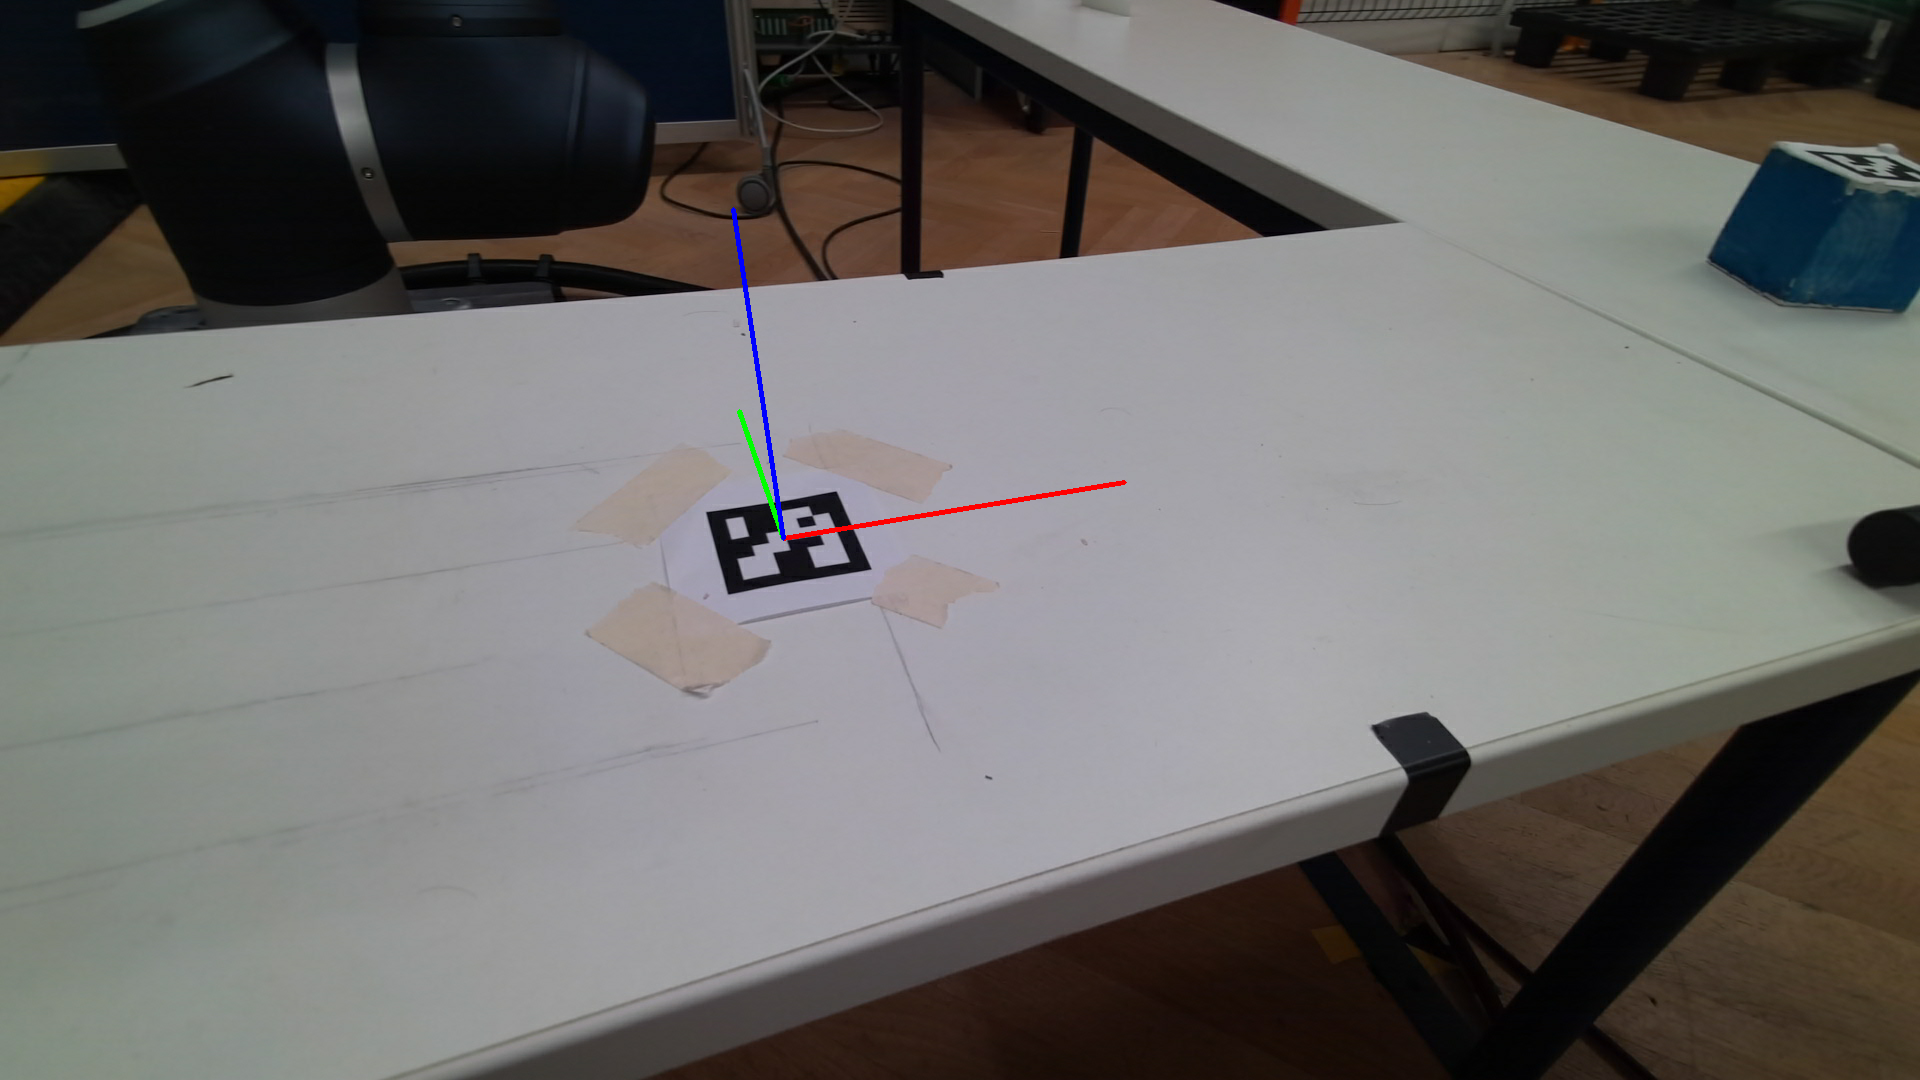
\includegraphics[width=0.6\textwidth]{output.png}
    \caption{An example of pose identification using ArUco markers.}
    \label{fig:arucoExample}
\end{figure}

Overall, non-learning based methods, while simple and computationally efficient, often require strictly controlled enviroments and specific conditions to be functional. This greatly restricts their applicability, and therefore learning-based methods are more widely used.

\section{Learning-Based Methods}
\label{s:learningbasedmethods}

Since the introduction of Convolutional Neural Networks (CNN), artifical intelligence and deep learning have been widely applied to the field of image processing, including its subfields of object detection and 6D pose estimation. The methods described in this section aim to train a CNN on vast quantities of data to perform a certain task. Based on the specifics of this task, we can categorize these approaches into three main branches: 2D-3D correspondence, direct estimation, and pose refinement. We will give a couple of examples for each of these categories.

\subsection{2D-3D Correspondence}
\label{ss:2D3D}

This class of methods uses a two step approach: they first implement a neural network to regress a set of 2-D points from an image, corresponding to a set of known feature points, and then use PnP to obtain the 6D pose of the object.

BB8\cite{BB8} uses object segmentation to perform 2D object detection, then regresses the 8 points that form the 3D bounding box of an object, but struggles with textureless symmetric or partially occluded objects. To combat these issues, PVNet\cite{PVNet} uses farthest point sampling to select keypoints on the surface of the object, and then implements a dense pixel-wise voting network, where each pixel "votes" on locations for the keypoints. RANSAC\cite{RANSAC} is then used to exclude outliers and obtain predictions with their probability distribution, which are then used for uncertainty-driven PnP.

Most approaches in this class share two common weaknesses. First, they are very perfomance-intensive when estimating the pose of multiple objects, since keypoint regression and PnP have to be computed for each object individually\cite{bukschat2020efficientpose}. Second, they are not end-to-end trainable, as the loss functions implemented do not reflect the final perfomance on the pose estimation task\cite{SS6D}. However, recent approaches have faced this issue by implementing learned or differentiable PnP algorithms, so as to enable end-to-end training\cite{EPro-Pnp}.

\subsection{Direct Estimation}
\label{ss:directestimation}

The approaches in this category exploit convolutional neural networks to directly regress the pose of an object in a single step. They are end-to-end trainable and boast better run times than the previously seen 2D-3D methods.

PoseNet\cite{PoseNet} was one of the first implementations of this concept, and was originally conceptualized for obtaining the camera pose from outdoor or indoor enviroments, and not for object pose estimation. Deep-6DPose\cite{deep6D} works by extending the Mask R-CNN\cite{Mask-R-CNN} instance segmentator, which in turn extends the Faster R-CNN\cite{Faster-R-CNN} object detector, and introduced a key technical feature by decoupling rotation and translation parameters, so as to make the pose regression loss differential. PoseCNN\cite{PoseCNN} expanded on this idea, and introduced a novel loss function that enabled it to properly handle symmetric objects.

Most networks in this category are fast and relatively accurate, but struggle in situations with partial occlusions.

\begin{table}[ht]
    \begin{center}
        \begin{tabular}{||c c c c c||} 
        \hline
        Rank & Model Name & Mean ADD & Method & Year\\ [0.5ex] 
        \hline\hline
        1 & RNNPose & 97.37 & Refinement & 2022 \\ 
        \hline
        2 & EfficientPose & 97.35 & Direct + Refinement & 2020 \\
        \hline
        3 & RePOSE & 96.1 & Refinement & 2021 \\
        \hline
        4 & EPro-PnP-6DoF v1 & 95.8 & 2D-3D & 2022\\
        \hline
        5 & ROPE & 95.61 & 2D-3D & 2021 \\
        \hline
        6 & DPOD & 95.2 & 2D-3D + Refinement & 2019\\
        \hline
        7 & HRNet  & 93.3 & 2D-3D & 2019 \\
        \hline
        8 & HybridPose & 91.3 & 2D-3D & 2020 \\
        \hline
        9 & CDPN & 89.86 & 2D-3D + Direct & 2019 \\
        \hline
        10 & PoseCNN + DeepIM & 88.6 & Direct + Refinement & 2018\\
        \hline
        \end{tabular}
    \caption{Top ten performing models on the LINEMOD dataset\cite{linemod} as of November 2022. Data taken from paperswithcode.com/sota/6d-pose-estimation-on-linemod.}
    \label{tab:top10models}
    \end{center}
\end{table}

\subsection{Pose Refinement}
\label{ss:poserefinement}

The previously explained algorithms may only give a rough estimate of the object pose at times. If greater accuracy is required, it is often necessary to use pose refinement algorithms. Approaches in this category start from an inital estimate, and then use various methods to refine it, obtaining a more accurate prediction.

DeepIM\cite{DeepIM} employs an iterative approach, by repeatedly rendering a 3D model of the object and matching it against the observed image. To ensure successive iteraterations gain in precision, it is trained not only on an annotated dataset, but also on previous outputs of the network. RNNPose\cite{RNNPose}, while also starting from a rendering and the observed image, formulates the task as a nonlinear optimization problem: it minimizes differences between correspondence fields by leveraging recent discoveries in the field of optical flow estimation, while recurrently calling itself. RNNPose currently boasts the best performance on the widely used LINEMOD\cite{linemod} dataset by a narrow margin, as highlighted by table \ref{tab:top10models}.

While refinement methods achieve remarkable performance, they have two main downsides. First, they rely on an inital estimate of the pose, so they cannot be applied independently, and second, they are relatively computationally intensive, especially when one considers that they must be run in parallel with another estimation method to generate the initial poses.

\begin{figure}[ht]
    \centering
    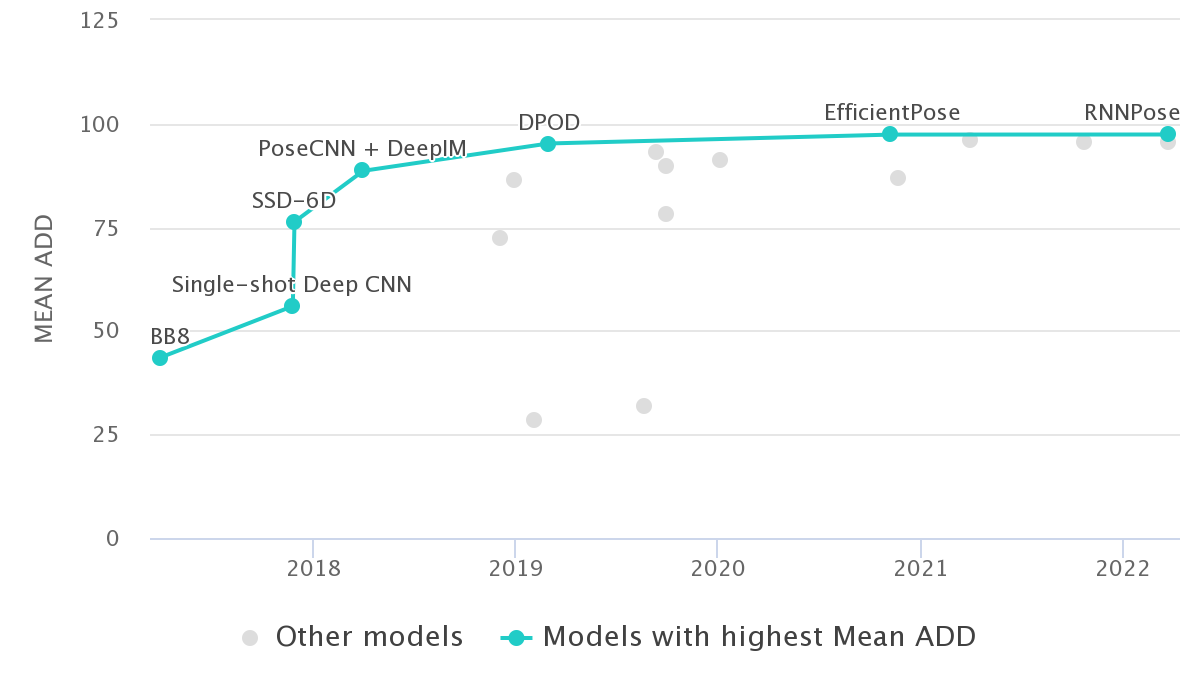
\includegraphics[width=0.7\textwidth]{linemodchart.png}
    \caption{Performance on LINEMOD of recent pose estimation algorithms by year. Graphic originates from paperswithcode.com/sota/6d-pose-estimation-on-linemod.}
    \label{fig:linemodchart}
\end{figure}

\subsection{Conclusions on Learning Approaches}

Data-driven models based on deep learning are more widely applied than non-learning-based models, as a large variety of approaches exists, and each approach brings its own distinct advantages. When choosing a model, special attention must be given to the application the model is destined for. For single object pose estimation, especially in highly occluded enviroments, 2D-3D methods are the best choice. For multi-object pose estimation, direct estimation methods provide greater computational efficency. Whenever greater accuracy is required, pose refinement algorithms offer the best results.

\chapter{Methodology}

In this chapter we will go over the methods used to build and train our own pose estimation model.

\section{Fully Rendered Datasets}

\subsection{Motivations and Objective}

We find ourselves in the situation where we want to train a 6D pose estimation model on a set of objects that is not present in any available dataset. Therefore the first essential step to developing our model is the creation of our own datasets for training and evaluation.

These datasets consist of a collection of images containing the object we wish to track, with associated ground truths encoding the pose of the tracked object for each image. Collecting this data in the real world is tedious and difficult, considering the number of samples required for deep learning, and that any errors or biases will strongly affect the perfomance of the trained model. 

One possible solution is to use rendering software, which can generate potentially infinite quantites of training images with associated, perfectly accurate ground truths. However, while a model trained on this data could function in simulation, we have no guarantee whether it would also function in real life. This is because a simulated sensor and simulated enviroment are unable to reproduce unmodeled physical effects and noise in the same way a real sensor would with a real environment. This issue, dubbed the "reality gap"\cite{domainRandomization2}, is recurring in any field which relies on simulations to supply data.

Domain Randomization\cite{domainRandomization} is one of the most utilised methods for solving this issue. It states that introducing sufficient variability in the simulated domain will allow the model to generalise to the real world with no additional training. This allows us to entirely skip the laborious data collection step and instead rely on a 3D model of the object we wish to track, which is usually readily available and accurate.

\subsection{Generation Methodology}
\label{ss:ScrewDataset}

To render the images for our dataset, we used the Unity Perception package\cite{unityPerception}, which integrates domain randomization features into its pipeline. Unity Perception works by simulating a scene, and then rendering each simulated frame from the perspective of a virtual camera. 

When setting up the simulation, we specify the number of iterations to simulate and the number of frames to render for each iteration. At the beginning of each iteration, we call a set of randomizers; each randomizer is a script that sets one of the domain variables for the iteration, such as the pose of an object or the colour of the light source. The scene is then updated according to the domain variables, rendered, and the associated ground truth saved.

\begin{figure}
    \centering
    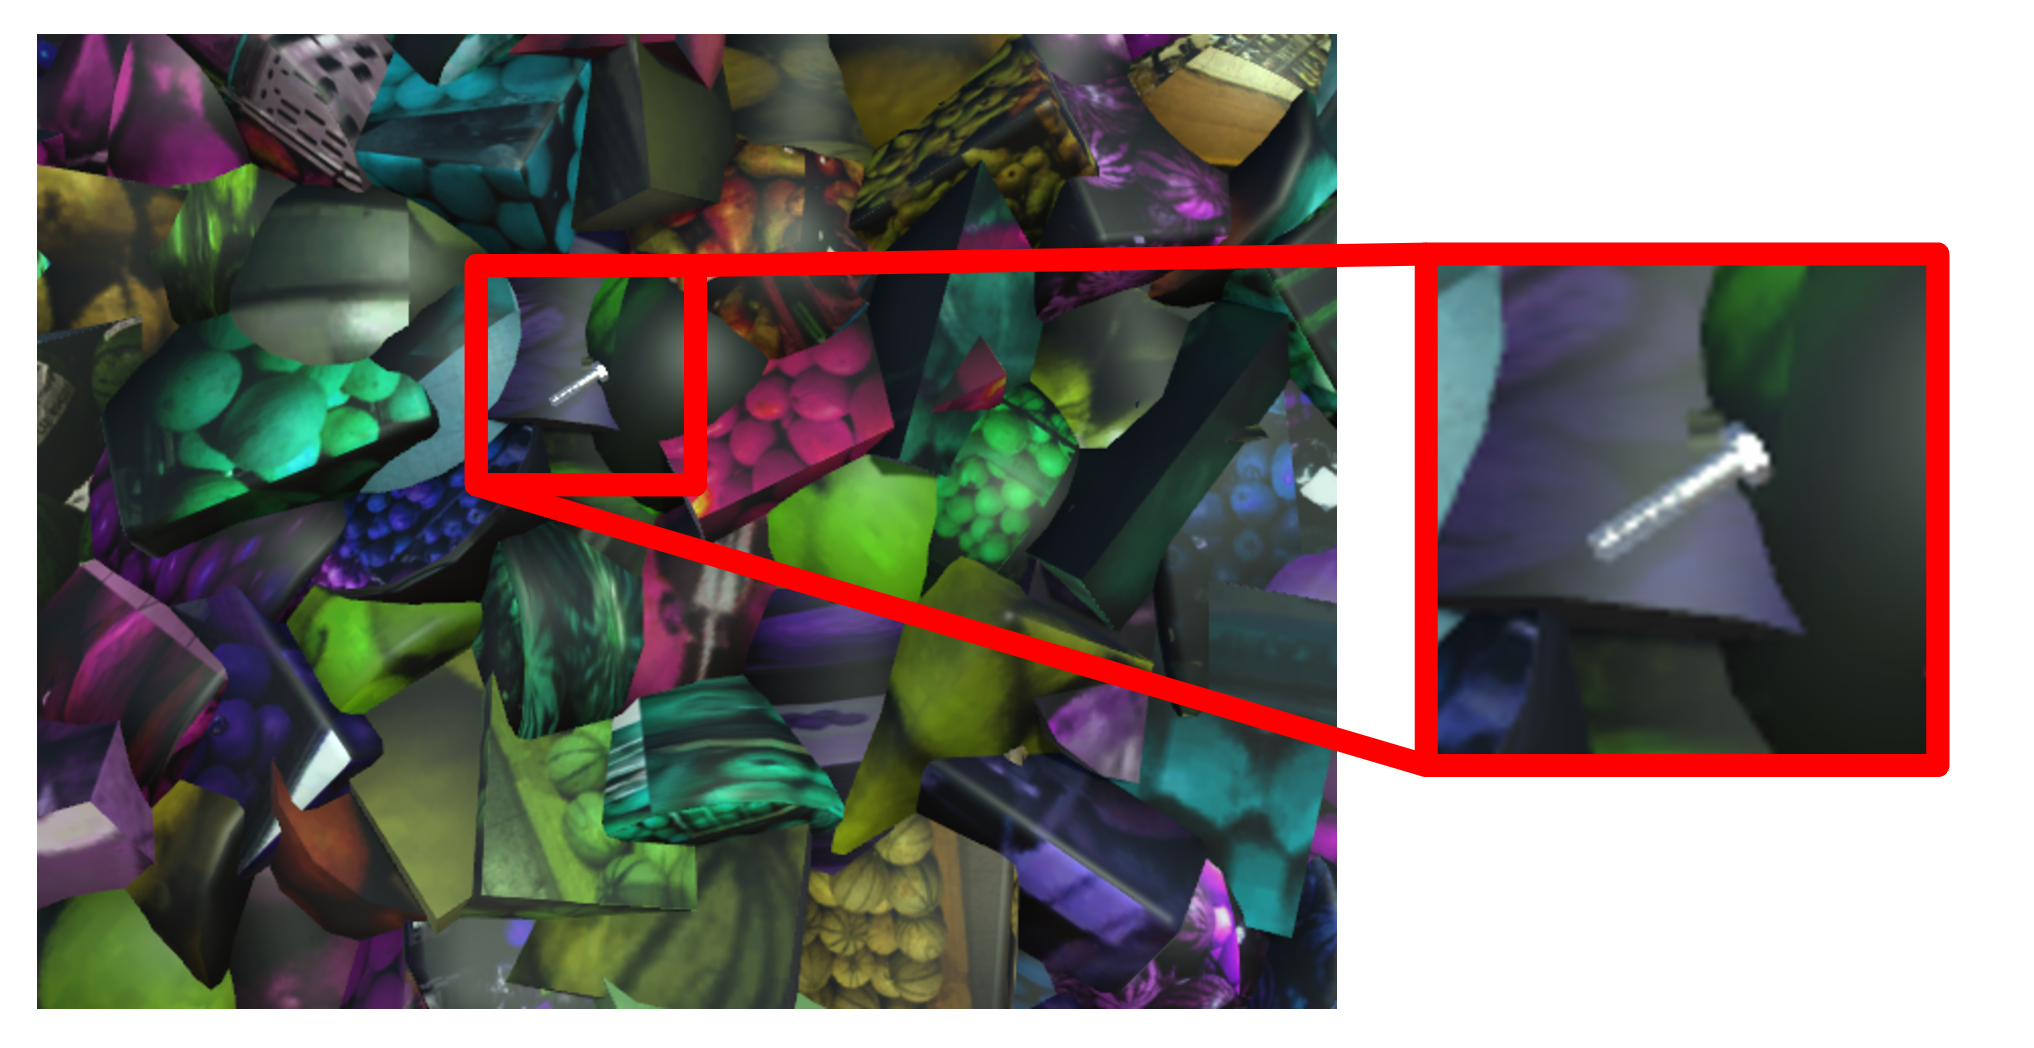
\includegraphics[width=0.6\textwidth]{screwdataset/ScrewDataset.png}
    \caption{One of the images generated with Unity's Perception package for training our model, with a zoom-in on the screw.}
    \label{fig:screwdataset}
\end{figure}

As a test case, we decided to generate a pose estimation dataset for a standard M6x30 hexagonal head screw. This is a very challenging object, as it is small and symmetric. The reason why symmetric objects are difficult for pose estimation is explained in depth in appendix A.2. The model of the M6x30 screw was obtained from the FreeCAD Fasteners workbench\cite{Fasteners} and colored with a metallic texture.

The domain for this dataset consists of images of the screw placed inside of a scene: thus the primary domain variables are the pose, the background, and the lighting. We used a custom randomizer to set position and rotation for each iteration, and default randomizers provided as part of the Perception package to generate a background, composed by random 3D shapes placed with random positions, orientations and textures. Finally, we used a custom randomizer to set the lighting color, intensity and origin. A sample image from this dataset appears in figure \ref{fig:screwdataset}.

We can then interface the output of this procedure with EfficientPose using a conversion script, which performs the necessary tasks to make the dataset compatible with the generators used by the network. In this manner we can quickly and easily generate arbitrarily large datasets for training, by first running the Unity scenario, and then running the conversion script for EfficientPose.

\subsection{Training}

The original version of EfficientPose is trained on LINEMOD. However, the specifics of LINEMOD and of our own dataset are widely different: LINEMOD has around 1200 images per object, and only about 200 of these are used for training, while our dataset has 10000 images, 9000 of which are used for training. This means that we must set proper training parameters for our own situation.

First, we reduced the number of epochs from 5000 to 100. Since our dataset contains 45 times more images, these two values represent a similar training time. EfficientPose also by default evaluates the model only every 10 epochs due to the small epoch size; we change this value to evaluate at the end of every epoch.

EfficientPose implements Keras' ReduceLRonPlateau callback to dynamically set the learning rate during training. This is standard practice: large learning rates quickly adjust the model but can lead to fluctuations, local minima and divergence; smaller learning rates avoid these issues but take an excessive amount of time to improve the model\cite{ReduceLR}. This method instead starts with a large learning rate, and then automatically reduces the learning rate whenever training stagnates, thus maintaining a value closer to the ideal. By default, EfficientPose halves the LR every time the accuracy does not improve for 25 epochs; we changed this to an 80\% reduction every 5 epochs, to account for the increased number of samples per epoch. The beneficial results of this process are visible in figure \ref{fig:screwdataset_training}: after epoch 27 the sudden drop in training and evaluation loss is due to a reduction in learning rate.

The initial and minimum learning rates are mantained identical to EfficientPose's, set at $10^{-4}$ and $10^{-7}$ respectively.

\subsection{Results}

\begin{figure}[ht]
    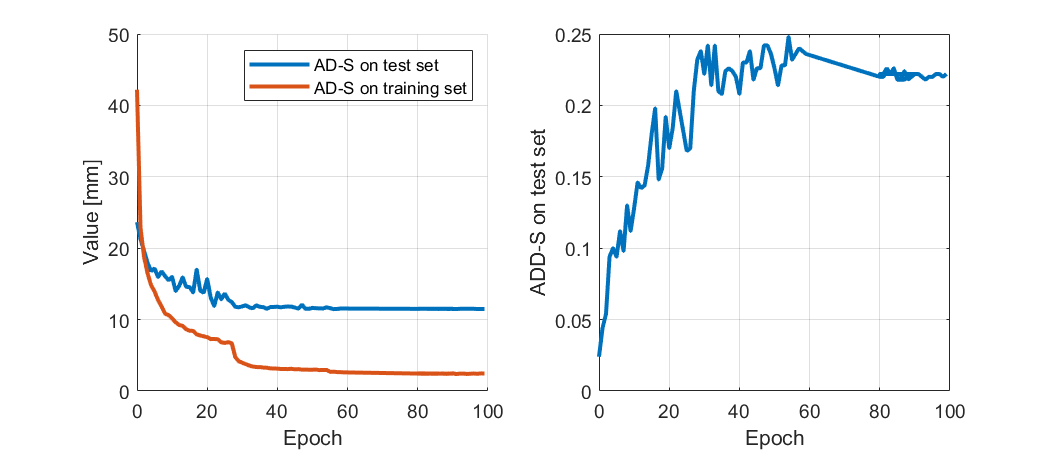
\includegraphics[width=\textwidth]{screwdataset_training.png}
    \caption{Evolution of the loss, AD-S and ADD-S metrics during training. The loss in this case is computed as the AD-S metric on the training dataset.}
    \label{fig:screwdataset_training}
\end{figure}

After 100 epochs of training, the progress of which is shown in figure \ref{fig:screwdataset_training}, the model has a final ADD of 22.2\%, with a peak value obtained during training of 24.8\%, much lower than the 97.35\% reported on LINEMOD. We can hypothesize that the reason for this performance gap is that the rendered dataset is much more difficult than LINEMOD, since we are dealing with a very small, symmetric object hidden inside a chaotic, colorful background with widely differing light conditions.

Another serious issue, that is more difficult to convey on paper, is that the model is not able to bridge the reality gap: while testing in real-life scenarios, it failed to identify the screw in most conditions, let alone produce accurate estimations. This means that it generalises poorly outside of the simulated environment, making it essentially unuseable.

\section{Partially Rendered Datasets}

\subsection{Motivations and Objective}

As stated above, the model trained on our custom dataset has very poor performance, both in simulated scenarios and in real-life applications. Since the same model has no similar issues when trained on LINEMOD, we can hypothesize that the cause lies with the training dataset itself, for two reasons:

\begin{enumerate}
    \item The training images are too difficult compared to the task we want to perform, preventing the network from learning properly.
    \item The training images and the real-life captures are excessively different, thus the model is not able to bridge the reality gap.
\end{enumerate}

The second issue is the most debilitating, as it makes whatever model we train completely unapplicable to any real life situation. We hypothesize that, since the backgrounds we generated are composed of a compact assortment of random shapes, with random sizes, colors, texures and poses, the resulting dataset is adeguate for representing extremely cluttered and noisy environments, but inadeguate for most other environments.

We have two options for facing this issue. The first would be to make the backgrounds more general in scope. This could mean, for example, generating a wider variety of synthetic backgrounds, or alternatively using sets of photographs, such as the COCO or Imagenet datasets, as other approaches have already done\cite{DPOD}. This would allow the model to generalise to more situations, including eventually our usecase. This is probably the best option if we forsee a wide application of the model in a variety of different conditions, for example in an autonomous driving scenario.

The second option is to generate a set of training images that more accurately depict a small number of chosen environments. This makes it easier for the model to bridge the reality gap by making this gap "smaller", reducing the differences between the training dataset and the typical image seen during inferencing. However, we have fewer guarantees on performance outside of the selected environments, which makes this approach better for usecases which are stationary or limited to fewer settings. This is often the case for industrial applications, making this second option our preferred choice.

Thus our objective is to create a method to easily and quickly generate a realistic training dataset for our testing environment, which is a simple table with the objects placed on its surface.

\subsection{Generation Methodology}

We again use Unity Perception to generate our training dataset, as described in \ref{ss:ScrewDataset}. We used models for 5 objects: the same M6x30 screw used previously, a M8x16 round head screw, a M8x25 and M8x50 socket head screws, and a M4x40 countersunk screw. As previously stated, these are small, symmetric objects that are generally challenging to identify, with the additional complication that they all have similar shapes and sizes. Only the first four  are annotated, while the M4x40 is included as a "decoy" to reduce the number of false positives.

The key issue now becomes the positioning of the objects in the image. Since in real-life conditions, the pose of an item is almost always influenced to some degree by its environment, we believe that simply placing the item freely in 6D space as we did in the previous approach would lose information compared to a realistic placement. Taking our example setting where the objects are placed on a surface, this constrains three degrees of freedom for each object: the vertical position relative to the surface, and the two rotations around the axises that determine the surface itself. Thus our objective is, for each image, to start from the pose of the surface relative to the camera, and from there generate a realistic pose for each dataset object, so that the object appears to be placed on the surface.

We thus captured a video of the testing table, which had been prepared with an ArUco marker in its centre. After eliminating blurry and off-center frames, we undistorted the images to obtain the set of backgrounds. Undistorting is an important step: it reduces the reality gap between the virtual sensor with no distortion and the real camera. To reduce it further, we set up the virtual sensor so that it imitates the parameters of the camera itself, an Azure Kinect sensor with a 1280x720 resolution and 90\degree field of view.

Once we have a set of background images, the placement surface in each image will be highlighted by an ArUco marker, thus we can easily obtain the position and rotation of this surface, as previously described in section \ref*{s:notlearningbasedmethods}. This results in a reference system corresponding to the marker, determined by a translation vector $t_s$ and a rotation matrix $\text{R}_s$, expressed relative to the camera reference system.

We then want to place the object's model with a random position and orientation on this surface. To do this, we can consider its pose relative to the marker reference system, which is given by a translation vector $t_r$ and a rotation matrix $\text{R}_r$. We can compute values of $t_r$ and $\text{R}_r$ considering the constraints of the surface:

\begin{equation}
    t_r = 
    \begin{bmatrix}
        x_r\\y_r\\0
    \end{bmatrix}
    ,\; \; \text{R}_r =
    \begin{bmatrix}
        \cos \theta_r & - \sin \theta_r & 0 \\
        \sin \theta_r & cos \theta_r & 0 \\
        0 & 0 & 1
    \end{bmatrix}
    \label{eq:translationsurface}
\end{equation}

... where $x_r$, $y_r$, and  $\theta_r$ are our three remaining free variables. We can extract their values from pre-defined probability distributions; in our case we used three uniform distributions $U(x_{min}$, $x_{max})$, $U(y_{min}, y_{max})$, and $U(\theta_{min}, \theta_{max})$. Essentially, \ref{eq:translationsurface} means that each object is free to translate along the surface, and to rotate around the axis perpendicular to the surface. Thus we can compute its pose $(t, \text{R})$ in the camera reference as:

\begin{align}
    t &= t_s + \text{R}_s t_r \label{eq:wrongpostionequation} \\
    \text{R} &= \text{R}_s \text{R}_r \nonumber
\end{align}

However, this operation alone is flawed, as it would place the origin of the 3D model on the surface, but for the objects in our dataset, the model origin is in the centre of the object. Therefore we must implement a final roto-translation that places the object on the surface starting from the position computed in \ref*{eq:wrongpostionequation}. This transformation differs based on the object, for example, if we consider the M6x30 screw, this correction transformation $(t_c, \text{R}_c)$ is given by a translation $z_c$ along the z-axis and a rotation by $\theta_c$ around the y-axis:

\begin{equation*}
    t_c = 
    \begin{bmatrix}
        0\\0\\z_c
    \end{bmatrix}
    ,\; \; \text{R}_c =
    \begin{bmatrix}
        \cos \theta_c & 0 & -\sin \theta_c\\
        0 & 1 & 0\\
        \sin \theta_c & 0 &  \cos \theta_c
    \end{bmatrix}
\end{equation*}

...where $z_c$ and $\theta_c$ depend on the dimensions of the screw as follows:

\begin{align*}
    \theta_c &= \frac{\pi}{2} - \arctan \frac{l_2}{l_1}\\
    z_c &= \frac{1}{2}d \sin \theta_c + \frac{1}{2} l \cos \theta_c
\end{align*}

The final pose in camera reference is then given by:

\begin{align*}
    t &= t_s + \text{R}_s t_r + \text{R}_s \text{R}_r t_c\\
    \text{R} &= \text{R}_s \text{R}_r \text{R}_c
\end{align*}

One thing to note is that if an object can have multiple positions on the surface, we consequently have multiple correction transformations to choose from. For example, each screw could be on its side or on its head, which implies a choice between two sets of $t_c$, $R_c$.

We implemented this method with Unity, using a custom randomizer that sets the pose of each object starting from the pose of the ArUco marker, which is pre-computed for each background image. We then have two more randomizers that set the background for each image and light intensity and rotation. A sample image from the final dataset is represented in figure TBA.

\subsection{Training}

The training dataset we generated has two major weaknesses. First, there is a limited number of background images, which means that the model has a finite number of camera positions to learn from, which in turn may lead to overfitting and unreliable results for positions that don't have sufficient representation. Second, it is difficult to randomize light intensity and color for the background images inside Unity, as it is decoupled from the same settings for the 3D models.

We can remedy these issues using data augmentation. This is a technique that involves applying random changes to data during training, similarly to how domain randomization would randomize them during generation. EfficientPose already provides two data augmentation methods: 6DoF and color. 6 Degree-of-Freedom augmentation involves randomly rescaling and rotating the input image and consequently adjusting the ground truth, so as to greatly increase the number of possible poses each image can provide. Color augumentation instead implements RandAugment\cite{RandAugment} to change the color and grain for the entire image. Applying both these methods results in images such as the one depicted in figure \ref{fig:ScrewPoseAugmented}, conveniently fixing the issues of our dataset.

Other training parameters are identical to the previous attempt with the fully generated dataset: 100 epochs, with an 80\% learning rate reduction if the model stagnates for 5 epochs.

\begin{figure}
    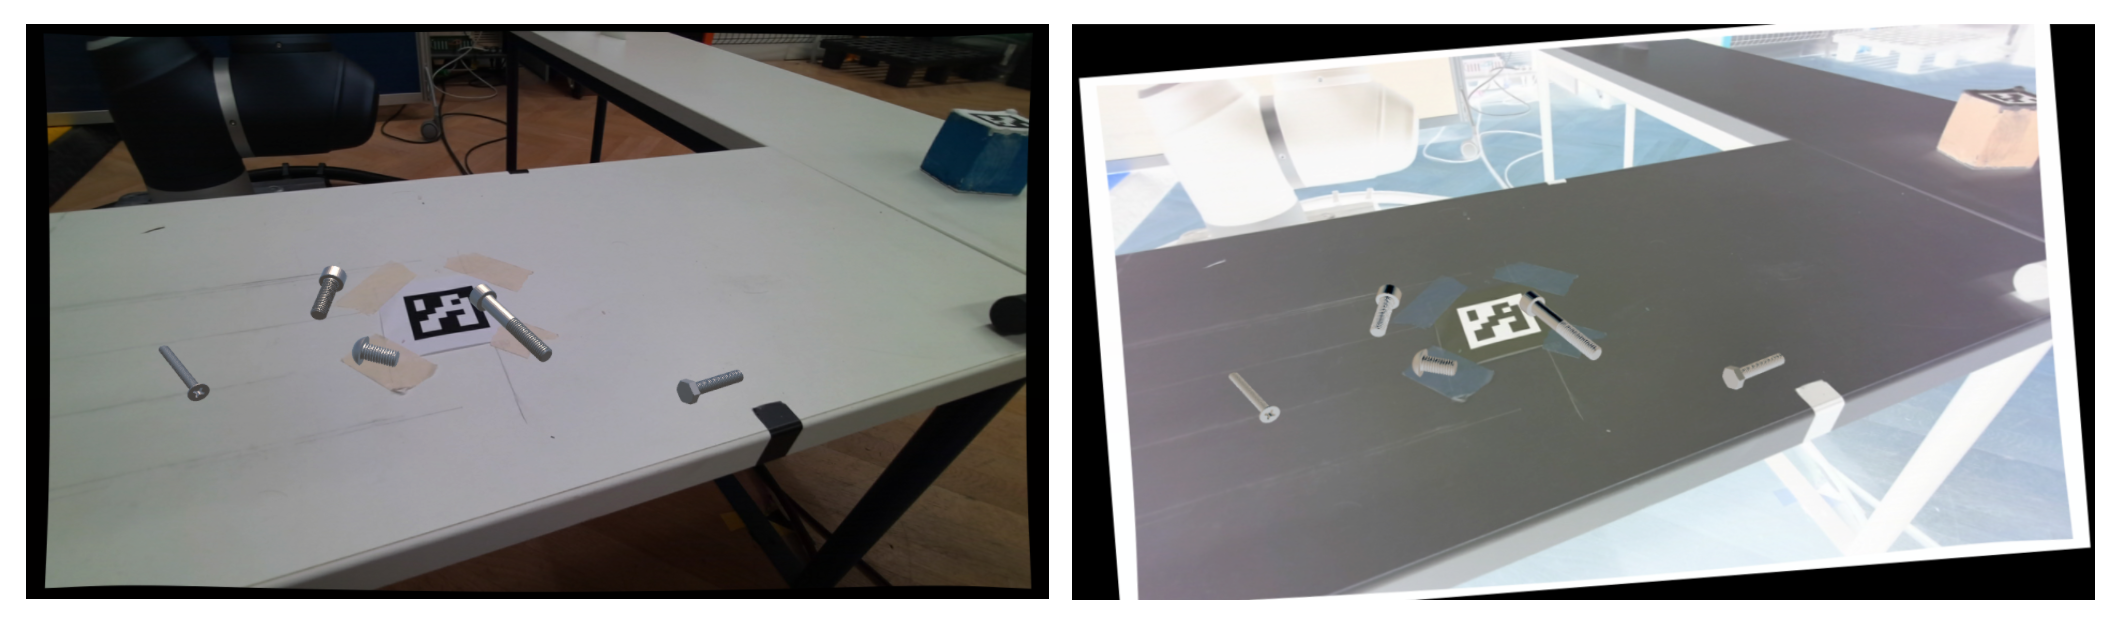
\includegraphics[width=0.7\textwidth]{screwposeaugmented.png}
    \caption{An example of a final training image resulting from data augmentation.}
    \label{fig:ScrewPoseAugmented}
\end{figure}

\subsection{Results}

\section{Semantics Applications}

\subsection{Motivations and Objective}

In many applications, it may be that estimating the pose of an object is sufficient to perform the task. However, in many situations it may be necessary to infer additional information from this data. An example may be the assembly of a workpiece from its components, where while tracking the pose of each individual component we may also have to track the state of the assembly itself.
\chapter{Results}

\section{Model Training Results}

In this section we will show progress and results of training the EfficientPose network on the three datasets presented in the previous chapter: the fully rendered dataset representing an M6x30 screw, henceforth referenced as "ScrewDataset", the augmented reality dataset representing a set of screws, henceforth "ScrewPose", and the augmented reality dataset representing the set of buttons and boards, henceforth "ButtonPose".

We will then be comparing these results with those obtained by EfficientPose on other datasets, namely LINEMOD for single object estimation and Occlusion-LINEMOD for multi-object estimation.

\begin{figure}[htp]
    \subfloat[Evolution using ScrewDataset for training.]{
        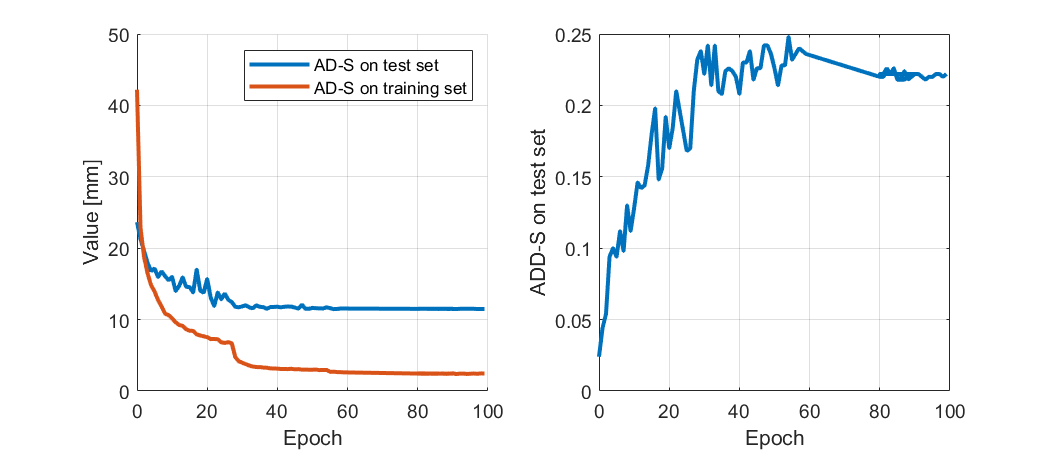
\includegraphics[width=0.8\textwidth]{screwdataset_training.png}
    }

    \subfloat[Evolution using ScrewPose for training.]{
        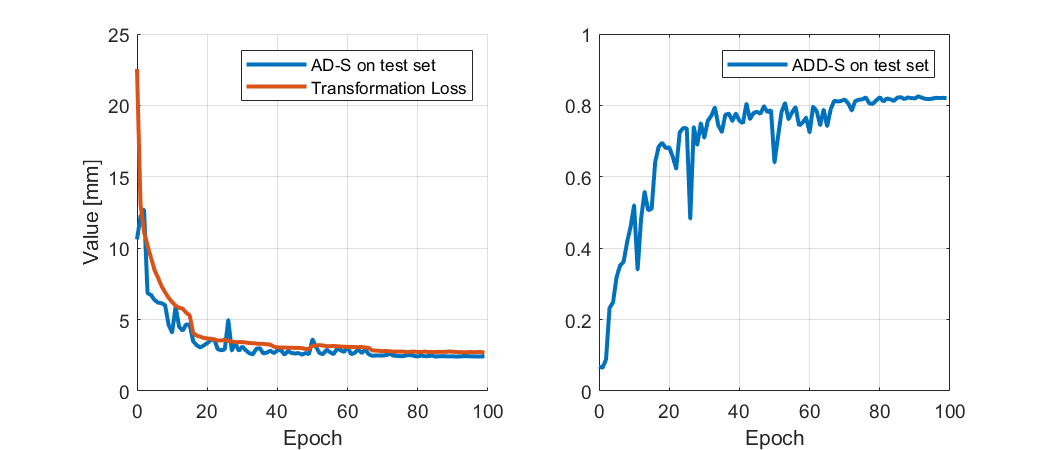
\includegraphics[width=0.8\textwidth]{screwpose_training.png}
    }

    \subfloat[Evolution using ButtonPose for training.]{
        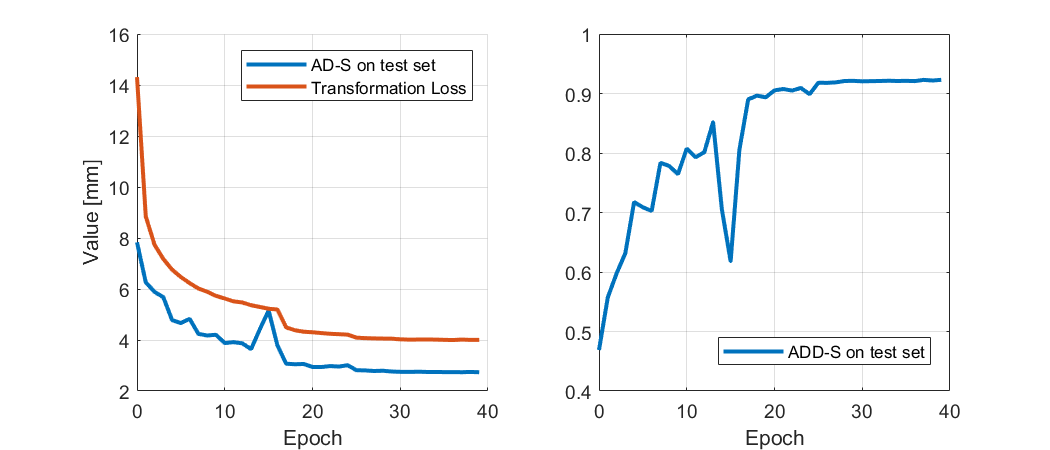
\includegraphics[width=0.8\textwidth]{buttonpose_training.png}
    }

    \caption{Training progress for EfficientPose on the ScrewDatset, ScrewPose and ButtonPose datsets, represented as the evolution of the transformation loss, AD-S and ADD-S metrics in evaluation for each epoch. Transformation loss is computed as the AD-S metric on the training dataset.}
\end{figure}

\begin{figure}[htp]
    \subfloat[ScrewDataset.]{
        \begin{tabular}{|c||c|c|c|}
            \hline
            Object & AP & AD-S [mm] & ADD-S \\
            \hline \hline
            M6x30 & 0.9675 & 11.4921 & 22.20\% \\
            \hline
        \end{tabular}
    }

    \subfloat[ScrewPose.]{
        \begin{tabular}{|c||c|c|c|}
            \hline
            Object & AP & AD-S [mm] & ADD-S \\
            \hline \hline
            M6x30 & 0.9399 & 2.1434 & 82.30\% \\
            M8x16 & 0.9538 & 1.9988 & 67.54\% \\
            M8x25 & 0.9645 & 2.1179 & 85.07\% \\
            M8x50 & 0.9880 & 3.4482 & 93.30\% \\
            \hline \hline
            Average & 0.9615 & 2.4271 & 82.05\% \\
            \hline    
        \end{tabular}
    }
    
    \subfloat[ButtonPose.]{
        \begin{tabular}{|c||c|c|c|}
            \hline
            Object & AP & AD-S [mm] & ADD-S \\
            \hline \hline
            2-slot & 0.9990 & 3.5420 & 99.90\% \\
            3-slot & 0.9985 & 3.9304 & 99.85\% \\
            red button & 0.9260 & 1.9825 & 86.01\% \\
            arrow button & 0.9349 & 2.0497 & 86.05\% \\
            safety button & 0.9962 & 2.6053 & 98.01\% \\
            unknown button & 0.9561 & 2.4757 & 82.95\% \\
            \hline \hline
            Average & 0.9685 & 2.76 & 92.13\% \\
            \hline    
        \end{tabular}
    }

    \caption{Evaluation of the Average Precision, Average Symmetric Distance, and ADD-S metrics on the ScrewDataset, ScrewPose and ButtonPose datasets after training.}
\end{figure}


On ScrewDataset, after 100 epochs of training the model has a final ADD of 22.20\%, with a peak value obtained during training of 24.8\%, much lower than the 97.35\% with $\phi=0$ reported by EfficientPose on LINEMOD. We can hypothesize that the reason for this performance gap is that the rendered dataset is much more difficult than LINEMOD, since we are dealing with a very small, symmetric object hidden inside a chaotic, colorful background with widely differing light conditions.

Another serious issue with this dataset, that is more difficult to convey on paper, is that the model is not able to bridge the reality gap: while testing in real-life scenarios, it failed to identify the screw in most conditions, let alone produce accurate estimations. This means that it generalises poorly outside of the simulated environment, making it essentially unuseable in real world applications.

On the flip side, the ScrewPose datset obtainined an average ADD-S of 82.05\%, which is better than EfficientPose's 79.04\% with $\phi=0$ on Occlusion-LINEMOD, and comparable to its 83.98\% with $\phi = 3$. This is a good result considering that the objects for our dataset are smaller, symmetric and all visually similar. Even though the Occlusion dataset is notoriously challenging, this anyways demonstrates the good performance of our own dataset. The model is also able to generalise to real life scenarios without noticeable losses in performance, as shown in figure \ref*{fig:inferencing}.

Finally, training on the ButtonPose dataset resulted in abnormally good performance for the boards, reaching over 99\% ADD-S and AP for both. The larger safety button also obtained great results, with a 98\% ADD-S, while the other buttons achieved more middling performances, but still better than the Occlusion-LINEMOD benchmark, showing that our approach is valid for more object sets. Noticeably, from this result and and the previous one it seems that performance for each object is proportional to its size: in both cases the network struggles with smaller objects (M8x16 screw, the smaller buttons), but performs much better with the larger ones (M8x50, the boards and larger safety button).

\begin{figure}[htp]
    \subfloat[ScrewPose.]{
        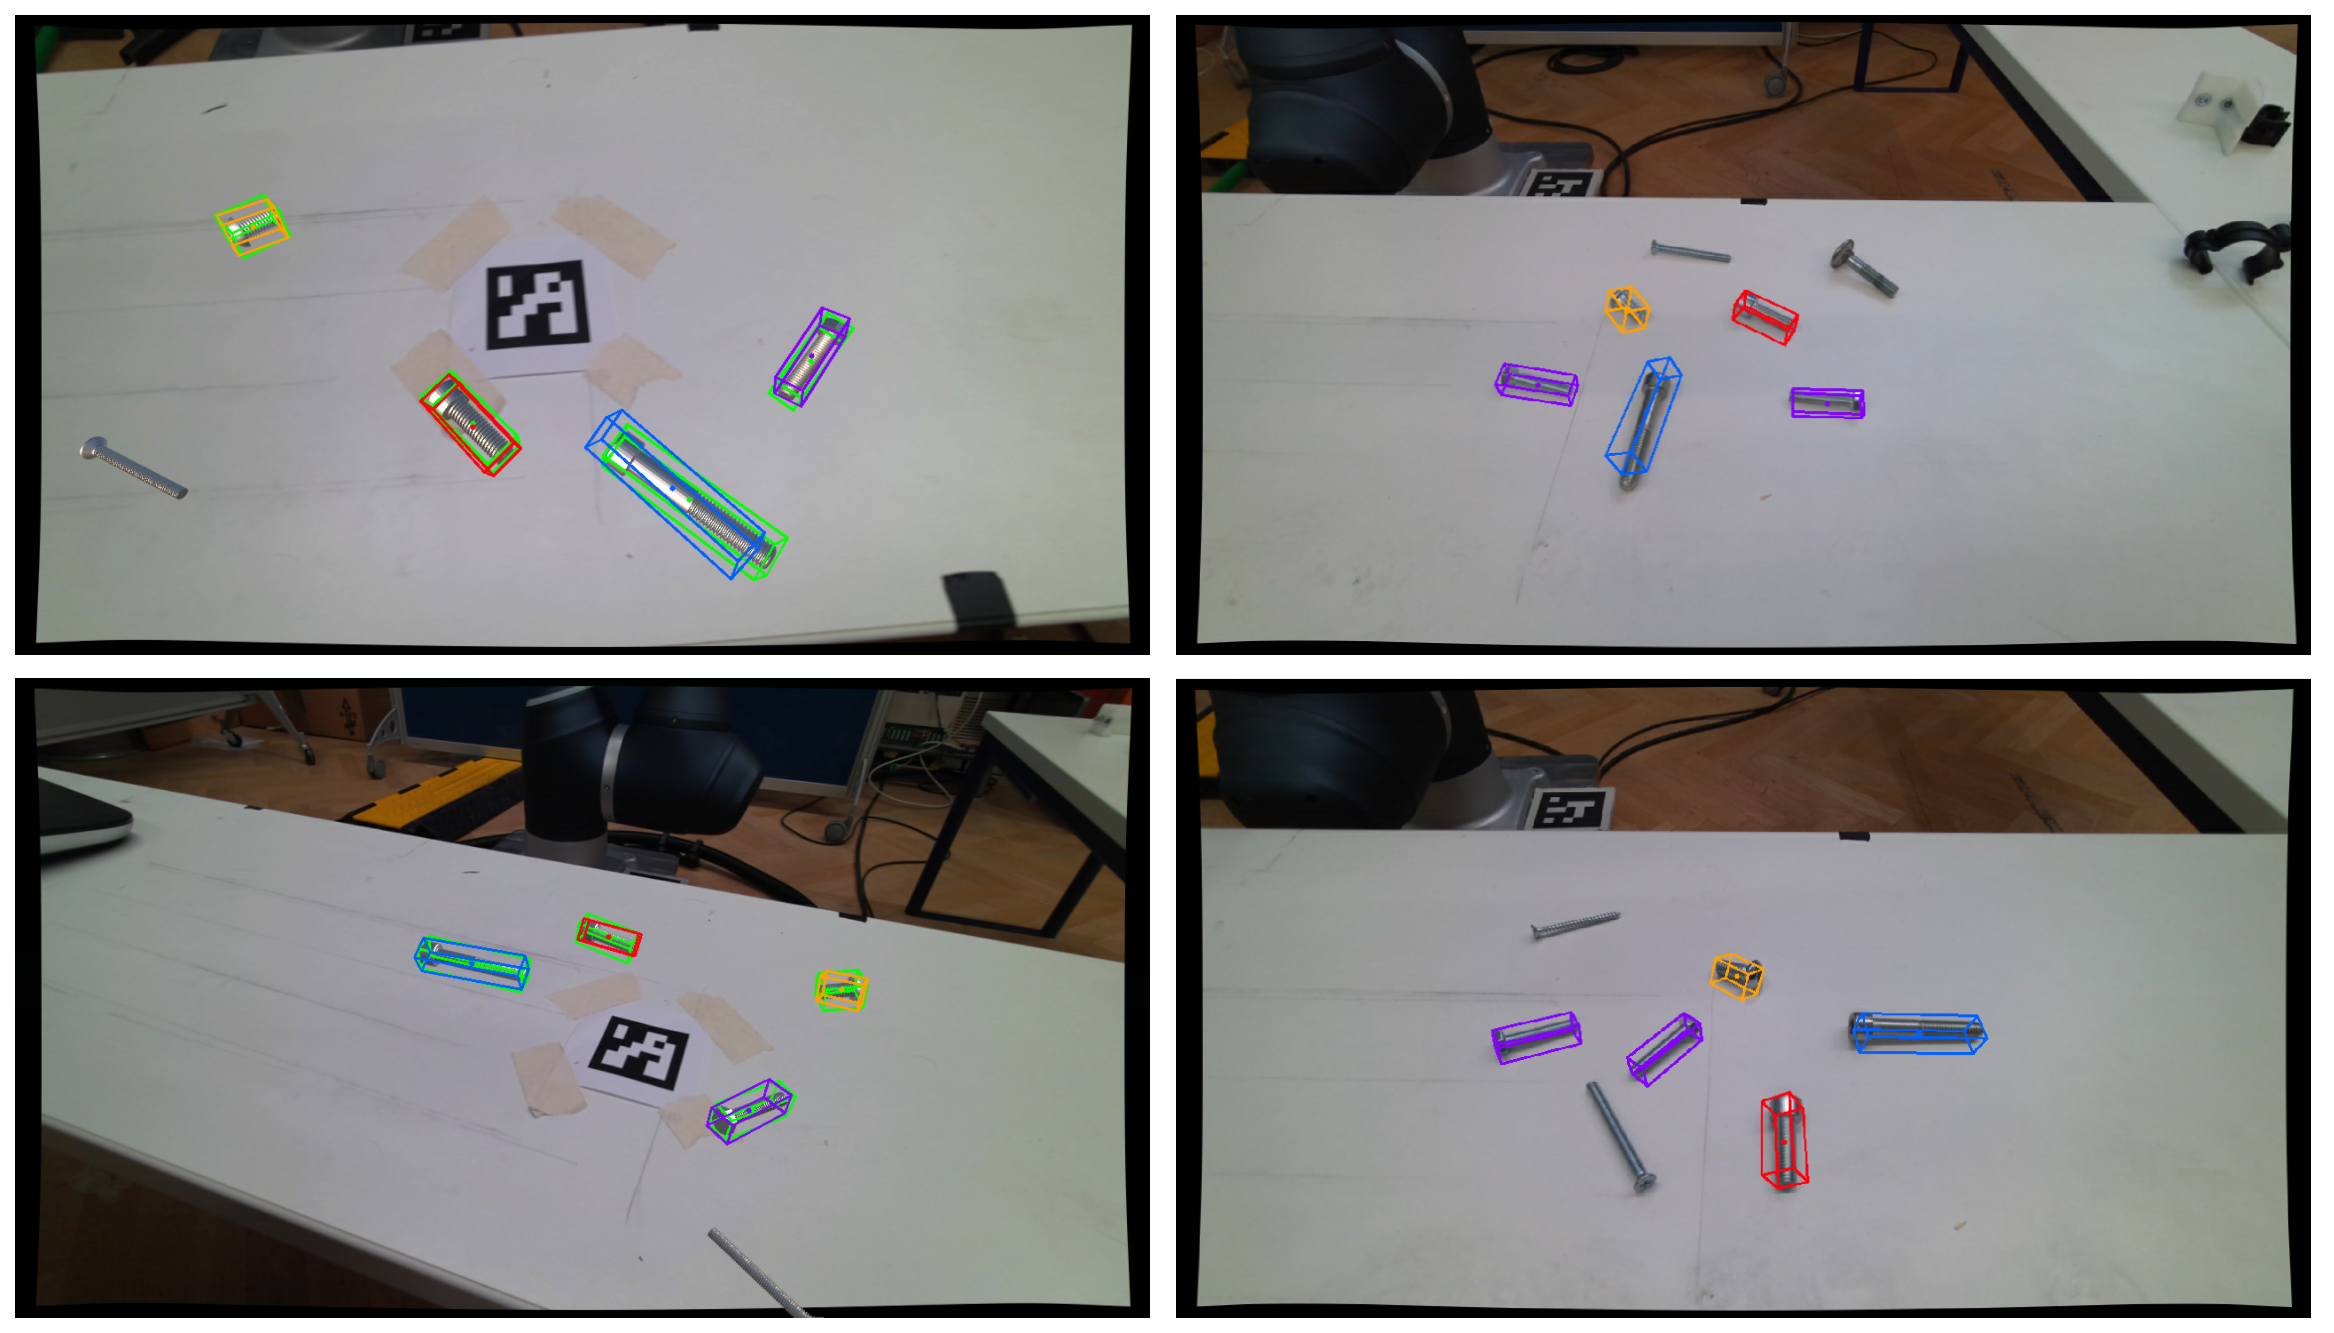
\includegraphics[width=\textwidth]{screwpose_inferencing.png}
    }

    \subfloat[ButtonPose.]{
        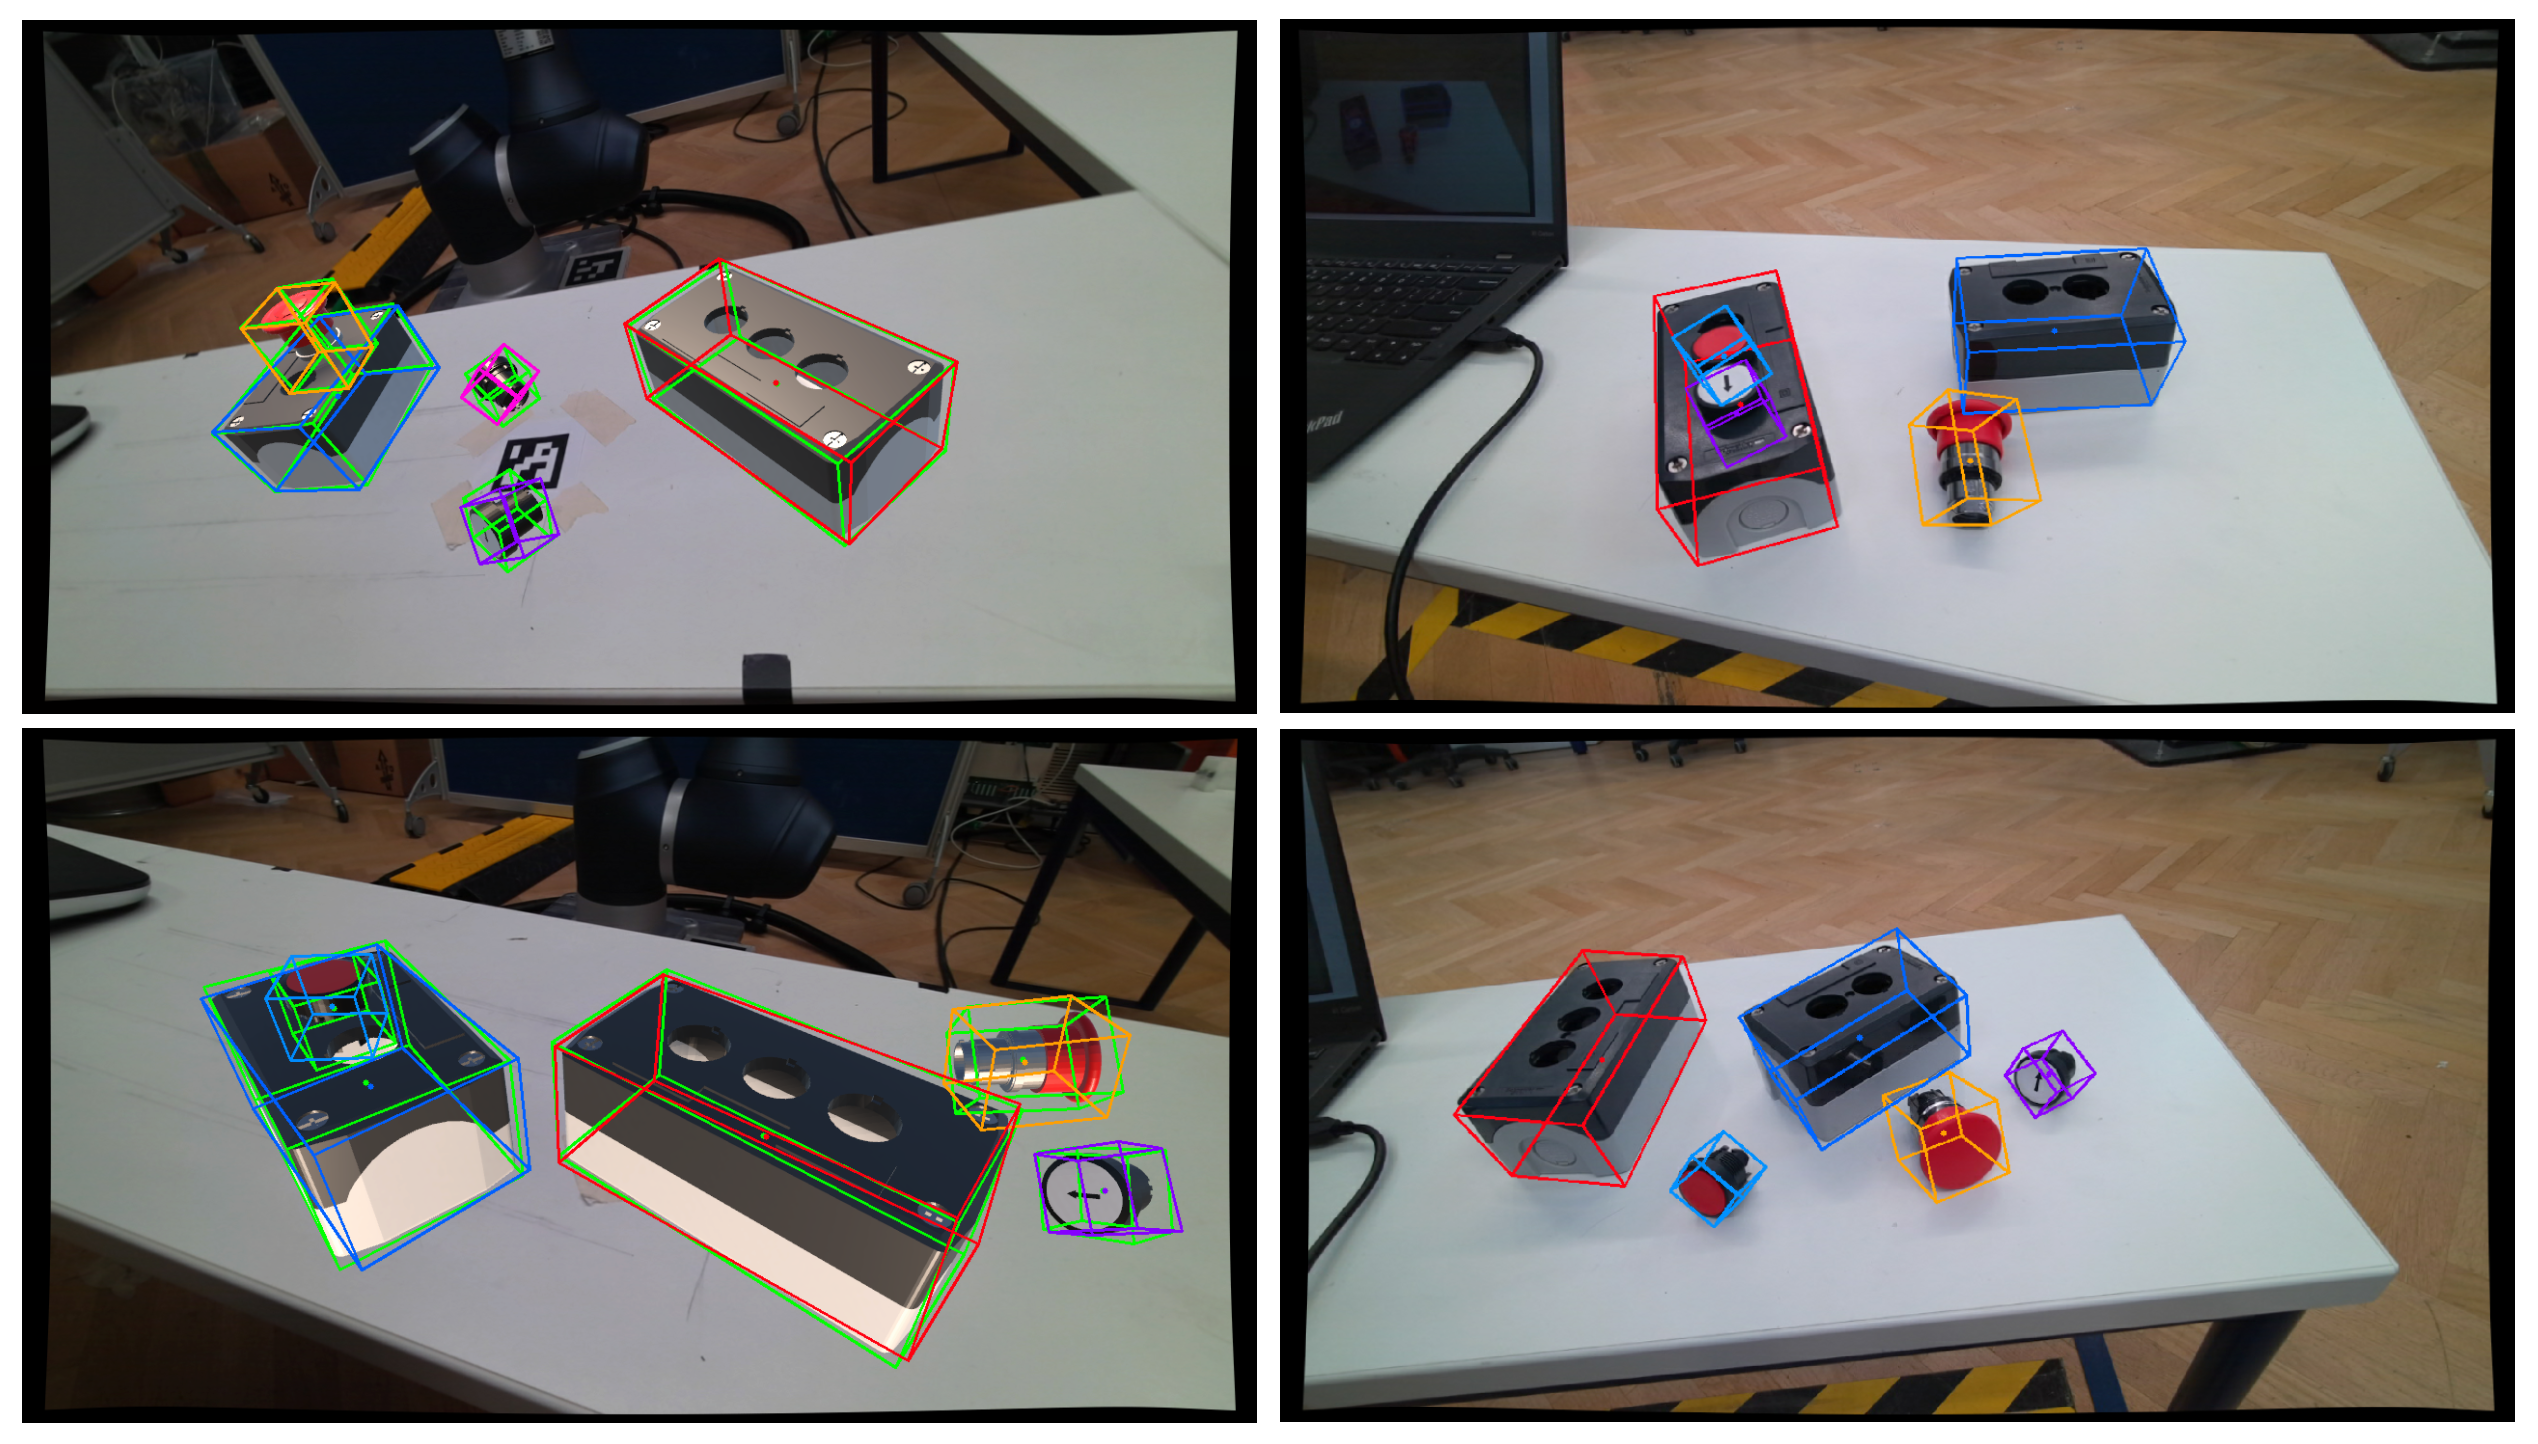
\includegraphics[width=\textwidth]{buttonpose_inferencing.png}
    }

    \caption{Images displaying pose estimations from the network for the ScrewPose and ButtonPose datasets. The left images are part of evaluation and display ground truths with green bounding boxes, the right ones are captures from a real camera in the testing environment.}
    \label{fig:inferencing}
\end{figure}

\Section{Impact of object dimensions and distance}

One noticeable result we observed after training was the impact that physical dimensions have on the final performance of the model for each object. Namely, larger and closer objects have much better performance than smaller and further objects. This is immediately noticeable in the ScrewPose dataset, where the larger M8x50 screw obtained the best results and the M8x16 obtained the worst.

To show how extreme these differences can be, we trained two additional models using new datasets based on the ButtonPose dataset. These two differ solely based on the background images: for the first one the backgrounds were captured from an approximate distance of 50 cm, while for the second one the backgrounds were captured from a distance of approximately 30 cm. For each of these conditions, we captured 50 backgrounds from a variety of positions at the same approximate distance from the marker. Our method for AR dataset generation proved to be a large asset in this, as creating these datasets was as simple as substituting the new backgrounds in the pipeline.

\Section{Semantic Meaning Extraction Results}

Given a binary classification problem such as ours (a button can either be in a slot or not), based on the output of our method we can build a confusion matrix as shown in table \ref{tab:cmatrix}.

\begin{table}[ht]
    \begin{center}
        \begin{tabular}{c||c|c}
            \space & Actual Positives & Actual Negatives\\
            \hline\hline
            Predicted Positives & True Positives (TP)& False Positives (FP)\\
            \hline
            Predicted Negatives & False Negatives (FN)& True Negatives (TN)\\
        \end{tabular}
        \caption{Generation of the confusion matrix.}
        \label{tab:cmatrix}
    \end{center}
\end{table}

We then define the precision and recall metrics as:

\begin{align*}
    \text{Precision} =& \frac{\text{TP}}{\text{TP}+\text{TN}} \\
    & \\
    \text{Recall} =& \frac{\text{TP}}{\text{TP}+\text{FN}}
\end{align*}

We want to maximise both of these metrics. To do this, we can plot them as a function of the threshold, and as a function of each other in a precision-recall graph, depicted in figure \ref{fig:precisionrecall}.

\begin{figure}[ht]
    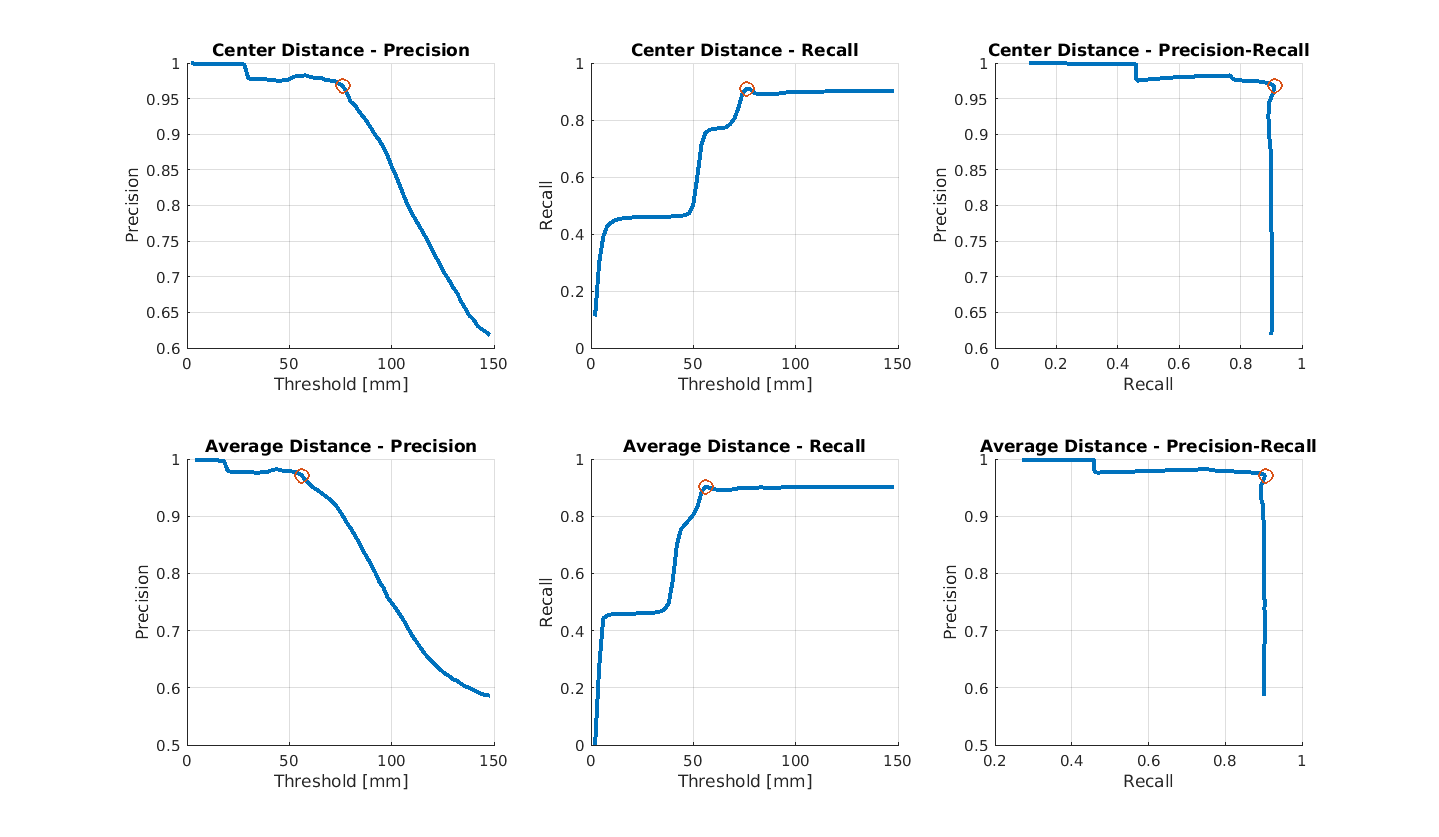
\includegraphics[width=\textwidth]{precision-recall.png}
    \caption{Precision and recall for both distance metrics on the Buttonpose dataset. The point with the best F1 score is highlighted with a red circle.}
    \label{fig:precisionrecall}
\end{figure}

As can be seen from the figure, higher thresholds greatly impact the precision of our model while lower thresholds greatly impact its recall. Overall we maintain high values, but our maximum recall is limited by the performance of the network to about 90\% for both distance metrics. To select the optimal threshold, we consider the F1 score, which is a balanced function of precision and recall:

\begin{equation*}
    \text{F1} = 2\times\frac{\text{Precision}\times\text{Recall}}{\text{Precision}+\text{Recall}}
\end{equation*}

For the average symmetric distance method, this results in a maximum F1 score of 0.9369, corresponding to a threshold of 56 mm, while for the center-to-center method the maximum is 0.9255, corresponging to a 78 mm threshold.

For our application we observe that there is no great advantage in using average distance over center-to-center. Given the additional complexity and computation time, the increase in performance is not significant.

We also obtained abnormally high thresholds for both methods. This can be attributed to the generated dataset: by stating that the buttons can only be either inside a slot or placed on the surface, we are in fact considering an ideal situation where a hypothetical manipulator does not commit any errors in picking up and inserting the buttons in their slots. If botched attempts are considered in the dataset, it is likely that the optimal threshold will be lower, and that the Average Distance method, being more sensible to situations with different rotations, may give better results than Center-to-Center.

Finally, the threshold is also influenced by the probability distribution we used for generating the poses for the button dataset, which in our case being a uniform distribution, resulted in a more spread-out placement, thus a higher optimal threshold. This is further compounded by the brute-force collision avoidance strategy implemented within the placement algorithm: if a placement attempt would generate an intersection with an already placed object, the placement was simply re-attempted from scratch. This naturally results in less conditions where dataset objects are in close proximity, and therefore in a higher threshold.



\chapter{Experiments and Evaluation Metrics}

In this chapter we will go over the various experiments and metrics used to evaluate the performance of our methods. This information is subsequently divided into three sections.

In the first section we will show the metrics used to describe the performance of the pose estimation network.

In the second section we will then show how we evaluated the performance of our semantic meaning extraction strategy.

Finally, in the third section we will discuss the experimental setup we used to test the performance of our complete model in a real-life robotics application.

\section{Evaluation Metrics for Pose Esitmation and Object Detection}

Most pose estimation and object detection methods share a common set of metrics on which their performance is evaluated. These are namely Average Precision for object detection strategies, and Average Distance and ADD for pose estimation strategies. In this section we will describe each metric, its meaning and how it is computed.

\subsection{Average Precision}

The performance of object detectors and 2D bounding box regressors is usually evaluated using median Average Precision (mAP), which is a descriptor of the reliability of a method's predictions. It exploits the intersection over union (IoU), computed as:

\begin{equation*}
    \text{IoU} = \frac{B_{GT} \cap B_{P}}{B_{GT} \cup B_{P}}
    \label{eq:IoU}
\end{equation*}

where $B_{GT}$ is the area of the ground truth bounding box and $B_{P}$ is the area of the network's predicion. A prediction is considered true if its IoU is greater than a threshold; based on this, we can generate the model's confusion matrix, as described in table \ref{confusionmatrix}.

\begin{table}[ht]
    \begin{center}
        \begin{tabular}{c||c|c}
            \space & Actual Positives & Actual Negatives\\
            \hline\hline
            Predicted Positives & True Positives (TP)& False Positives (FP)\\
            \hline
            Predicted Negatives & False Negatives (FN)& True Negatives (TN)\\
        \end{tabular}
        \caption{Generation of the confusion matrix.}
        \label{confusionmatrix}
    \end{center}
\end{table}

This matrix is the basis for the definition of the precision and recall metrics. Precision is an indicator of how well the model avoids false positives, while recall is an indicator of how well a model avoids false negatives. They are computed as follows:

\begin{align*}
    \text{Precision (P)} &= \frac{\text{TP}}{\text{TP} + \text{FP}}\\
    \text{Recall (R)} &= \frac{\text{TP}}{\text{TP} + \text{FN}}
\end{align*}

Precision and recall both depend on the value of the threshold: smaller thresholds will result in a more restrictive model, thus less false positives and more false negatives, high precision and low recall, while high thresholds will result in the opposite: more false positives, less false negatives, low precision and high recall.

It is common practice to plot the precision as a function of the recall in what is called a precision-recall curve, $P = f(R)$. Each point in the curve represents a value of the threshold, corresponding to its own confusion matrix and subsequent metrics. An example plot is shown in figure \ref{example_pr}.

\begin{figure}[ht]
    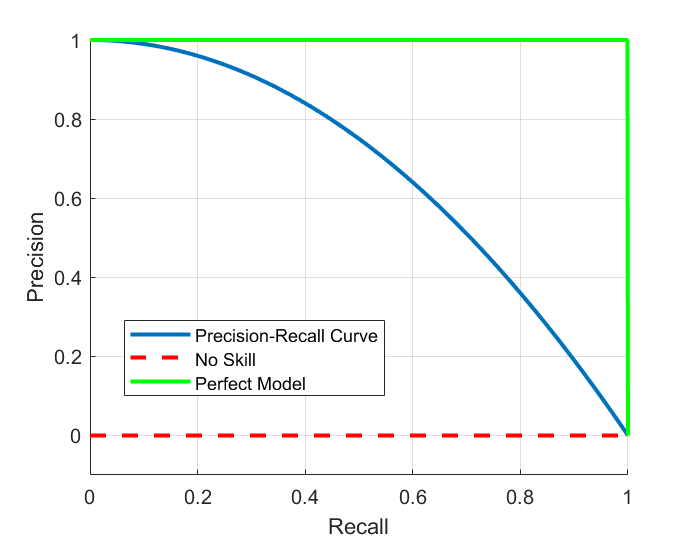
\includegraphics[width=0.6\textwidth]{example_pr_curve.png}
    \caption{Example of precision recall curves. The red line indicates a model with no skill at a task, thus zero precision; the blue line a model with some skill; the red line is the ideal behavior with maximum precision and recall at all times.}
    \label{example_pr}
\end{figure}

At this point we can describe the Average Precision (AP) as the mean value of the precision, corresponding to the area under the precision-recall curve:

\begin{equation*}
    \text{AP} = \int_{0}^{1} f(R)dR
\end{equation*}

The median Average Precision is then obtained as the average AP over all object classes:

\begin{equation*}
    \text{mAP} = \frac{1}{n} \sum_{i=1}^{n} \text{AP}_{i}
\end{equation*}

Therefore it is a real value between 0 and 1, with 0 representing the model with no skill, and 1 representing the ideal behavior.

\subsection{Average Distance and ADD}

Evaluation of pose estimation methods is almost exclusively done using the ADD metric, and by extension the Average Distance (AD). While the first is an indicator of the percentage of correct estimations, similar in a sense to mAP, the second is instead unique to pose estimation.

Given $n$ points belonging to the 3D model $M$ of an object, the AD represents the average of the distance between these points transformed according to the ground truth ($\text{R}, \text{t}$) and according to the prediction ($\hat{\text{R}}, \hat{\text{t}}$):

\begin{equation*}
    \text{AD} = \frac{1}{n} \sum_{x \in M} ||(\text{R}x + \text{t}) - 
    (\hat{\text{R}}x + \hat{\text{t}})||_2
\end{equation*}

The ADD is then given by the percentage of correct poses given by the model. A pose is correct if its AD metric is less than 10\% of the 3D model's diameter.

This metric has been in use since before the introduction of neural networks to pose estimation, but it runs into serious issues when dealing with objects that have rotational symmetry. The reason for this is that these objects may present no visual differences with different rotations. For example, one image of the M6x30 screw we use for inferencing could correspond to six different poses, each varying 60\degree from the previous one. This means that the model will eventually stabilize at a value that minimizes the average error, which is ususally large.

To combat this issue, we use the Symmetric Average Distance (AD-S)\cite{PoseCNN} metric, defined as the average minimum distance between points in the predicted pose and the ground truth:

\begin{equation*}
    \text{AD-S} = \frac{1}{n} \sum_{x_1 \in M} \min_{x_2 \in M} ||(\text{R}x_2 + \text{t}) - 
    (\hat{\text{R}}x_1 + \hat{\text{t}})||_2
\end{equation*}

This is very similar to the loss used in the ICP algorithm, as it only considers the distance from each point to its closest correspodent in the ground truth. Analogously to ADD, we then implement ADD-S as the percentage of correct poses.

Finally, we can introduce the Mixed Average Distance, which is defined as:

\begin{equation*}
    \text{ADD(-S)} = 
    \begin{cases}
        \text{ADD-S} & \text{if the object is symmetric,}\\
        \text{ADD} & \text{otherwise.}
    \end{cases}
\end{equation*}

We would like our model to have the highest possible ADD, however in an industrial environment it is important to also evaluate the AD. This is because for larger objects the ADD will tolerate greater estimation errors, as it is based on the diameter of the objects; these errors however may not be compatible with the precision required for a determined task.

\section{Semantics Evaluation Methodology}
\label{semantics_method_section}

To evaluate our semantic meaning extraction method, we must compare ground truth values for the semantic state of each scene, associated with its own image, with the outputs of our method.

Our strategy therefore is to save the semantic state for each image during dataset generation. We then run the trained model on a subset of these images, coinciding with the test set, to obtain predictions, and then run our semantic meaning extraction method on the predictions.

However, an issue arises from the application of this method. Due to the symmetry of the boards, it is impossible to determine visually which slot is which. For example in figure \ref{sym_eval}, the ground truth is that there is a button in the first slot, however the model outputs the button in the second slot. Visually, both of these interpretations are correct, since the board is symmetrical, however directly comparing the output with the ground truth results in two "false" values.

\begin{figure}[ht]
    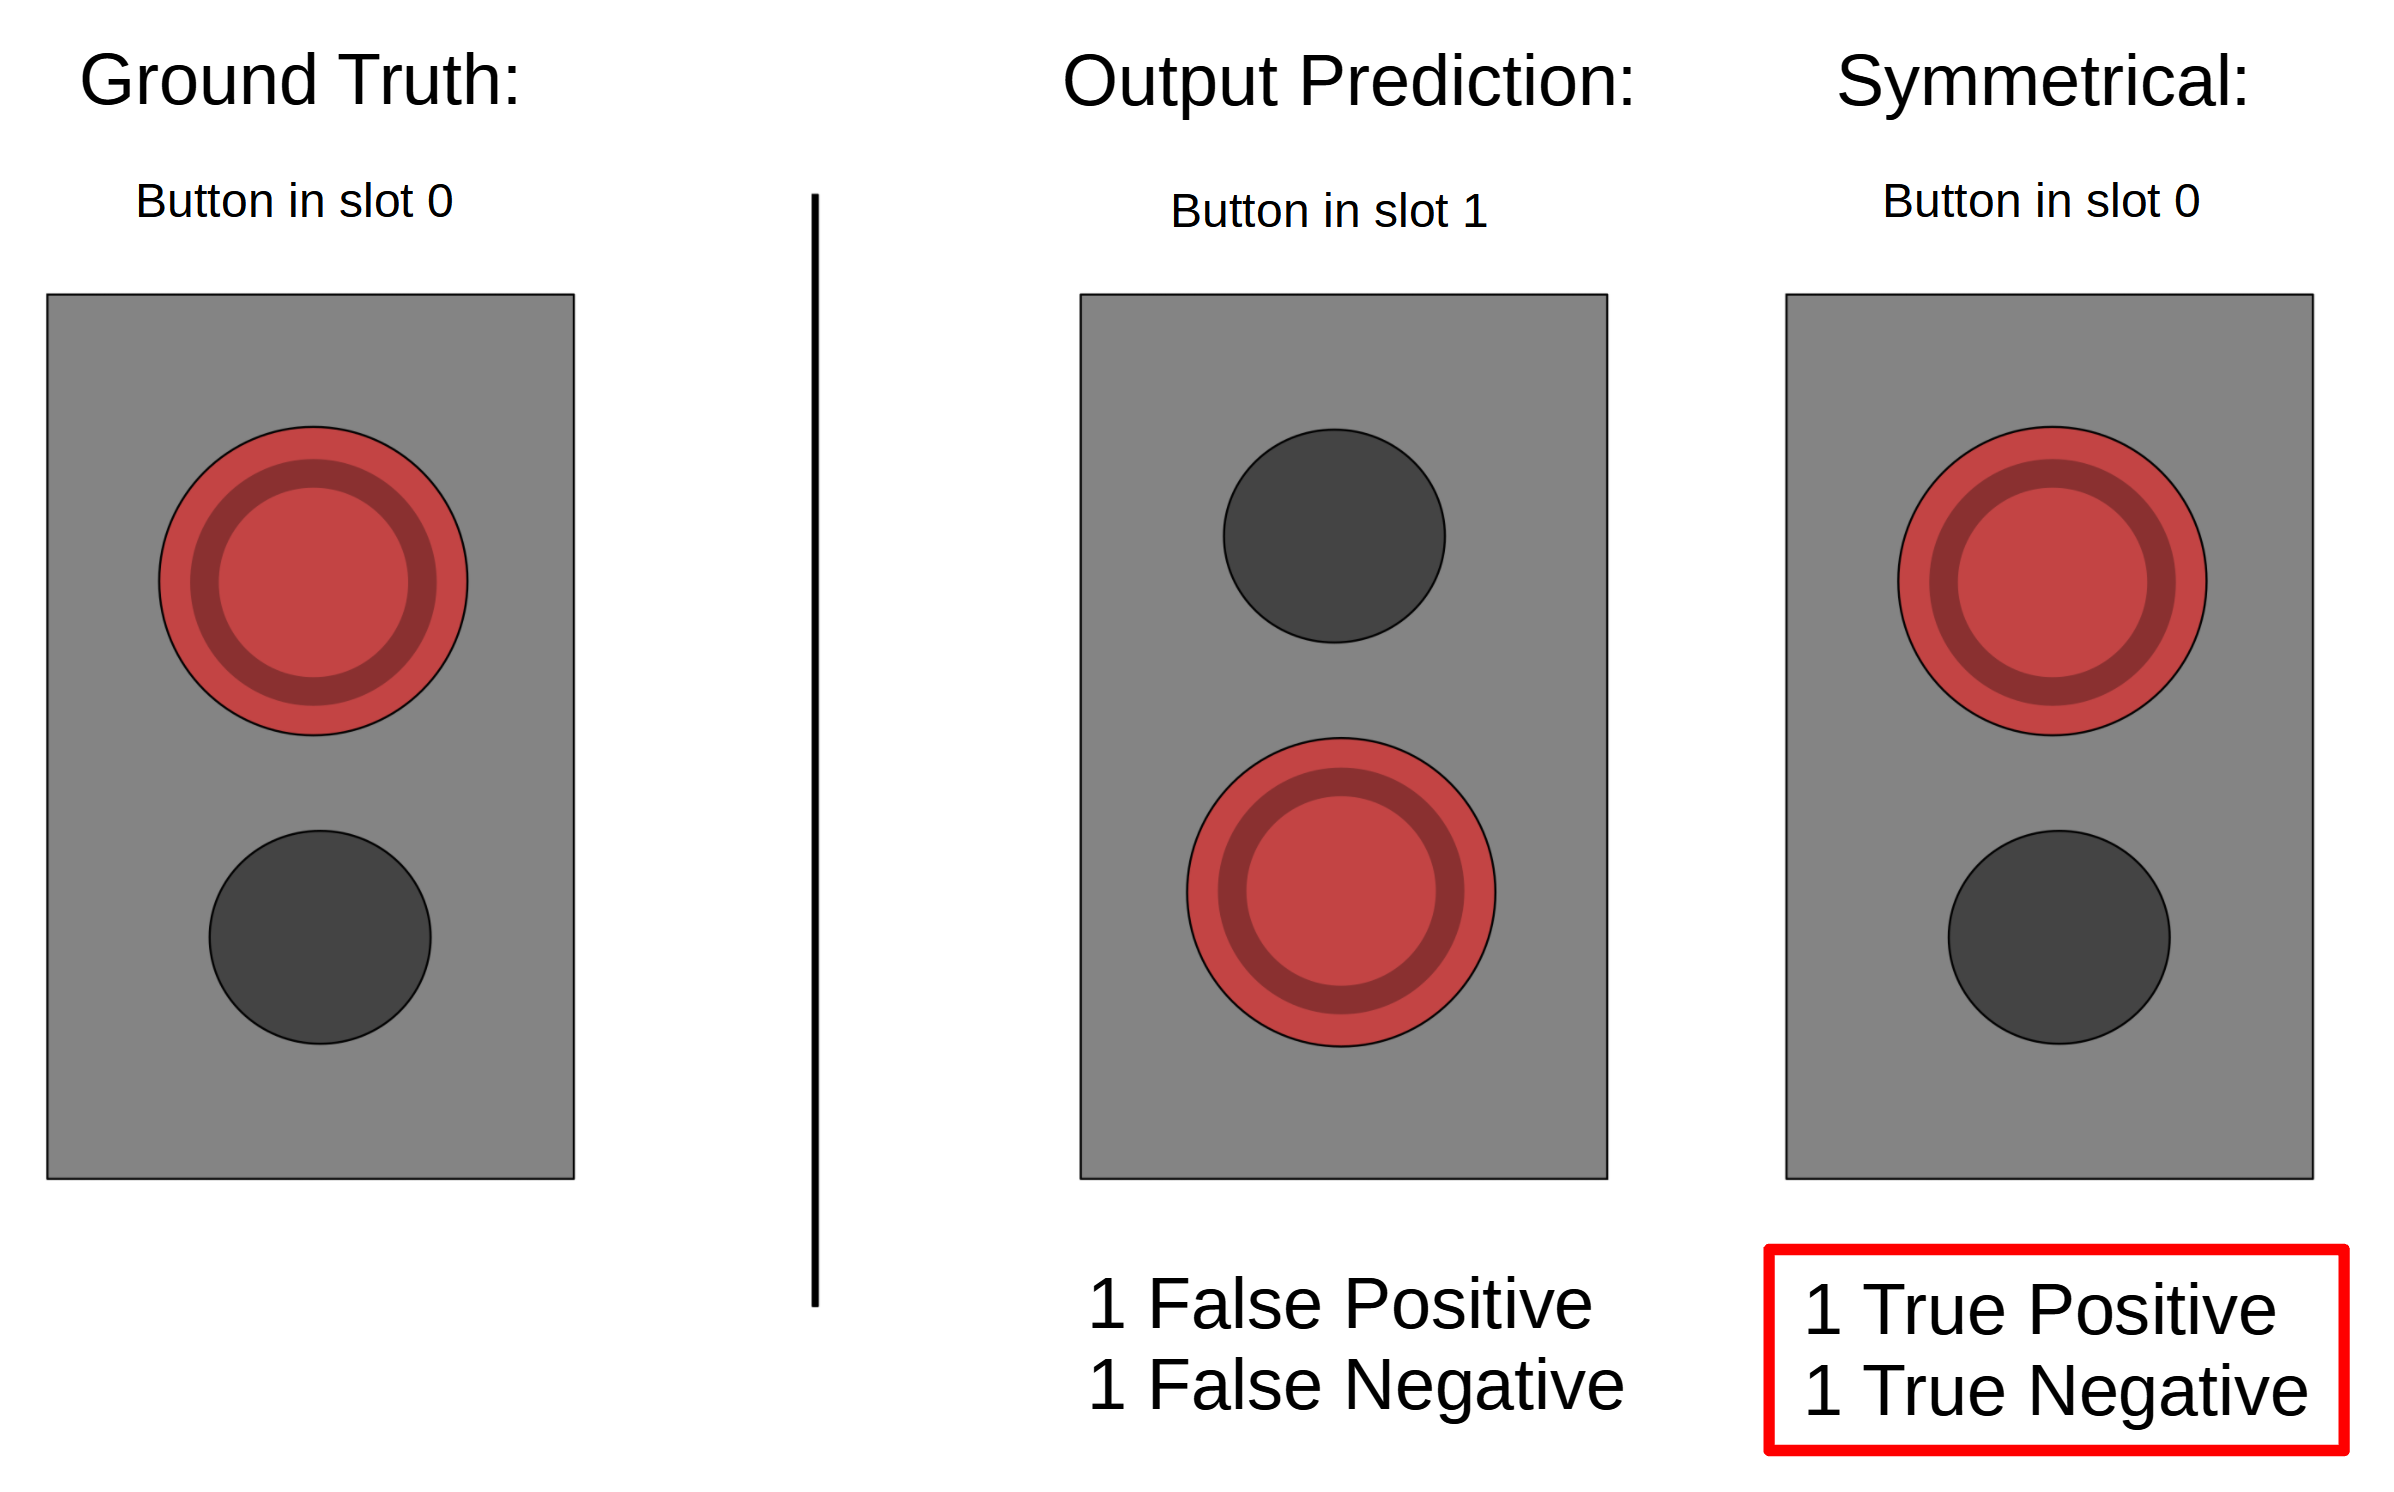
\includegraphics[width=0.8\textwidth]{sym_evaluation.png}
    \caption{Selection between the model's output and its symmetrical when evaluating the semantic state of a scene.}
    \label{sym_eval}
\end{figure}

To combat this issue, we consider both the model's output, and its symmetrical condition, and take the results from the version with the greatest number of true values when compared with the ground truth. Therefore we compare both the model output and its symmetrical: since the symmetrical results in two "true" values, the final output of the comparison is two "true" values: a true negative and a true positive.

Once this issue has been resolved, we can build for each given threshold a confusion matrix as described in the previous section, and compute a precision-recall curve.

To select the optimal threshold, we consider the F1 score, which is a balanced function of precision and recall, computed as:

\begin{equation*}
    \text{F1} = 2\times\frac{\text{Precision}\times\text{Recall}}{\text{Precision}+\text{Recall}}
\end{equation*}

We consider the optimal threshold to be the one that maximises this value.

\begin{figure}[ht]
    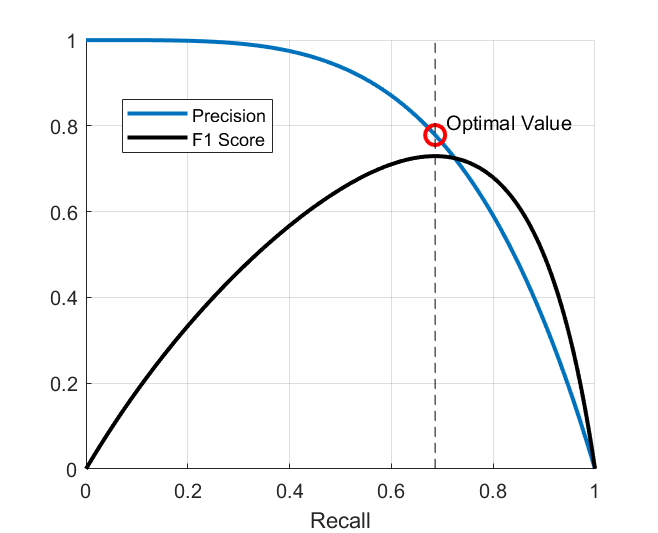
\includegraphics[width=0.5\textwidth]{best_f1_example.png}
    \caption{Example of selecting the optimal threshold using the maximum of the F1 curve.}
\end{figure}

\section{Real-Life Experimental Setup}

To test the effectiveness of our vision and semantics model, we will be implementing it in a real life situation where we have to complete a simple assembly task. We will be using a Doosan A0509s robotic manipulator equipped with a pneumatic gripper, and an Azure Kinect camera. We will be re-utilizing previously developed code for this system that generates behaviour trees \cite{behavior_tree} to drive the robot based on previous demostrations of actions and their effects on the scene.

First, we must describe each scene using a list of predicates. These predicates are first-order logic functions that can be either true or false, and must be evaluated each time we obtain new information on the scene. A list of these predicates and their descriptions is supplied in figure \ref{predicateslist}.

\begin{table}[ht]
    \begin{center}
        \begin{tabular}{cc}
            Predicate & Description \\
            \hline \hline
            IsGripperEmpty(gripper) & True when no objects are in the gripper. \\
            \hline
            IsGrapsed(Button, Gripper) & True when the button is grasped by the gripper. \\
            \hline
            IsButtonInSlot(Button, Slot) & True when the button is inserted in the slot. \\
            \hline
            IsSlotEmpty(Slot) & True when no buttons are in the slot.\\
        \end{tabular}
        \caption{List of predicates used to describe scenes in our application, with descriptions.}
        \label{predicateslist}
    \end{center}
\end{table}

Once these predicates are available and can be evaluated, we can "teach" the robot to perform actions through kinesthetic demostrations. During these demostrations, the robot, moved by a human operator, will modify the environment and thus change the state of the scene. Since this state can be described using a list of predicates, we can save the differences between the inital state and the final state to understand the pre-requisites and consequences of each action in predicate form. We then use Planning Domain Definition Language (PDDL) \cite{pddl} to define each action and unite these definitions into a domain description. For example, if we take our task of picking up a button and inserting it into a slot, the states would be as described in figure \ref{predicatesevolutions}.

\begin{figure}[ht]
    \subfloat[Initial State]{
        \begin{tabular}{c}
            Predicates: \\
            \hline
            IsSlotEmpty(slot) \\
            IsGripperEmpty(gripper) \\
            ... \\
        \end{tabular}
    }

    \subfloat[Intermediate State]{
        \begin{tabular}{c}
            Predicates: \\
            \hline
            IsSlotEmpty(slot) \\
            IsGrasped(button, gripper) \\
            ...\\
        \end{tabular}
    }

    \subfloat[Final State]{
        \begin{tabular}{c}
            Predicates: \\
            \hline
            IsButtonInSlot(button, slot) \\
            IsGripperEmpty(gripper) \\
            ...\
        \end{tabular}
    }

    \caption{Evolution of the state, expressed as a list of predicates, during the pick-up and insertion of a button into a slot.}
    \label{predicatesevolutions}
\end{figure}

The domain for this task would then contain a list of the possible predicates, and two actions: the evolution from the initial state to the intermediate state (picking up the button) and the evolution from the intermediate state to the final state (inserting it into the slot), shown in figure \ref{pddlactions}.

\begin{figure}
    \subfloat[action_0 (Picking up a button)]{
        \begin{tabular}{c|c|c}
            Parameters & Preconditions & Effects \\
            \hline
            gripper & IsGripperEmpty(gripper) & !IsGripperEmpty(gripper) \\
            button & \space & IsGrasped(button) \\
        \end{tabular}
    }
    \subfloat[action_1 (Inserting a button into a slot)]{
        \begin{tabular}{c|c|c}
            Parameters & Preconditions & Effects \\
            \hline
            button & IsGrasped(button) & !IsGrasped(button) \\
            slot & IsSlotEmpty(slot) & !IsSlotEmpty(slot) \\
            gripper & \space & IsGripperEmpty(gripper) \\
            \space & \space & IsButtonInSlot(button, slot) \\
        \end{tabular}
    }

    \caption{Actions with their parameters, preconditions and effects as saved by PDDL for our task.}
    \label{pddlactions}
\end{figure}

We then define an init and goal for our planner, which are the state we are starting from and the final state we want to achieve, compact both of these into the "problem definition". Inputting the definition and the domain into a PDDL planner then gives us the set of actions we need to perform, (in this case action_0 and the action_1), which we can use to then build our behaviour tree.

The main modification applied to the previous code in this approach, apart from changing the predicates to suit our needs, is the shift from a continuously evaluated model to a discretely evaluated model. The reason for this change is the susceptibility of the vision model to false positives for previously unidentified objects. More information on this can be found in section \ref{false_positives_issue}, but essentially in this manner we ensure that the state is evaluated only when the gripper and eventual human operator are outside of the camera's field of view.


\chapter{Results}

In this chapter we will go over the results we obtained by testing our methods.

In the first section we will show the results of training the EfficientPose network on our datasets, and subsequent observations. In the second section we test the performance of our semantic meaning extraction strategy. Finally, in the third section we show how effective our overall system is in a real-world robotics application.

\section{Model Training Results}

In this section we will show the results of training the EfficientPose network on the three datasets presented in the previous chapter: the fully rendered dataset representing an M6x30 screw, henceforth referenced as "ScrewDataset", the augmented reality dataset representing a set of screws, henceforth "ScrewPose", and the augmented reality dataset representing the set of buttons and boards, henceforth "ButtonPose".

\begin{figure}[htp]
    \subfloat[Evolution using ScrewDataset for training.]{
        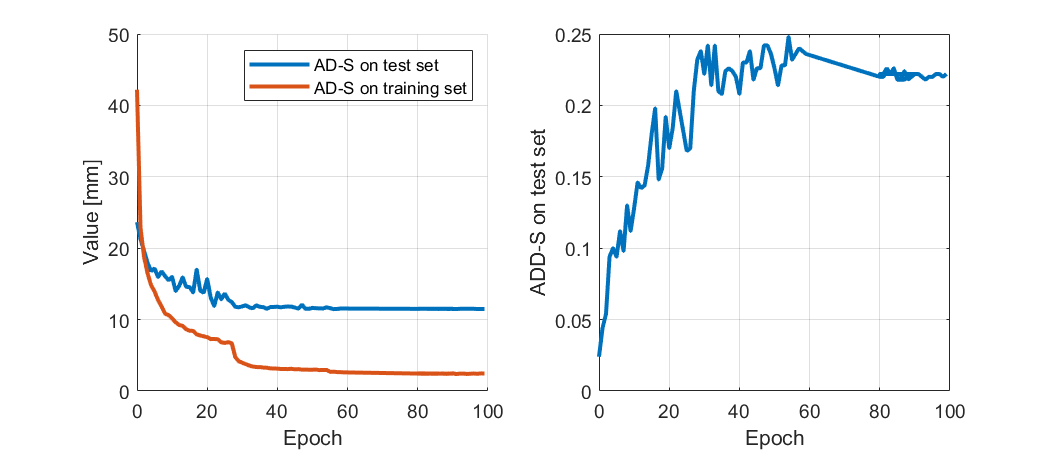
\includegraphics[width=0.7\textwidth]{screwdataset_training.png}
    }

    \subfloat[Evolution using ScrewPose for training.]{
        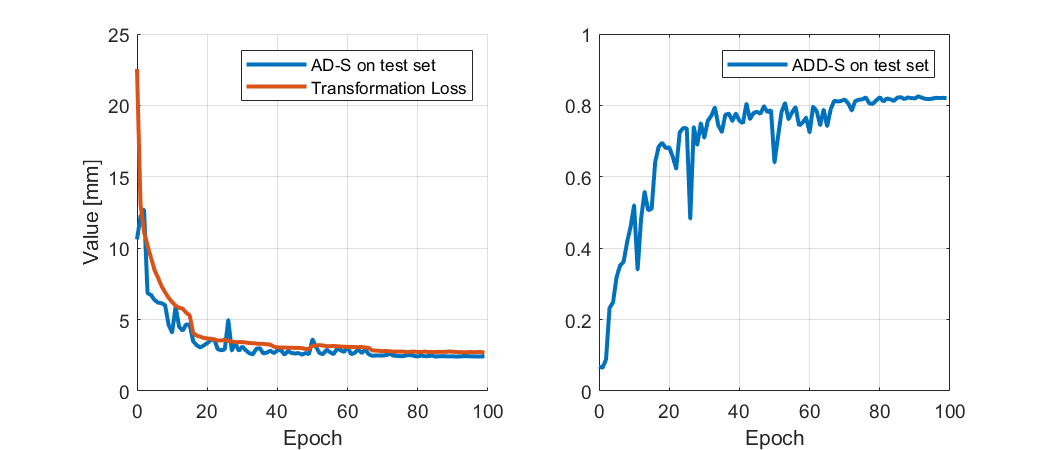
\includegraphics[width=0.7\textwidth]{screwpose_training.png}
    }

    \subfloat[Evolution using ButtonPose for training.]{
        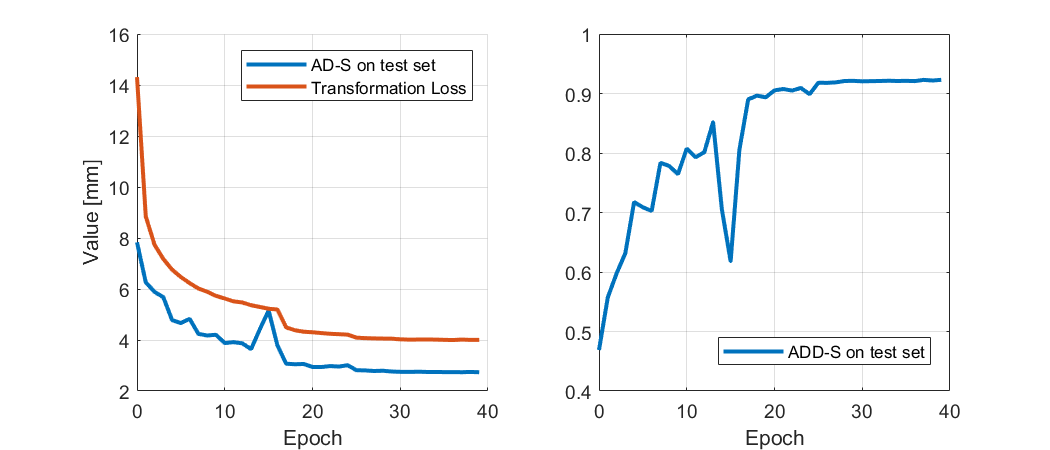
\includegraphics[width=0.7\textwidth]{buttonpose_training.png}
    }

    \caption{Training progress for EfficientPose on the ScrewDatset, ScrewPose and ButtonPose datsets, represented as the evolution of the AD-S and ADD-S metrics in evaluation for each epoch.}
    \label{fig:training_progress}
\end{figure}

We will then be comparing these results with those obtained by EfficientPose on other datasets, namely LINEMOD for single object estimation and Occlusion-LINEMOD for multi-object estimation.

The evolution of the loss and ADD-S metrics during training for these three datasets is shown in figure \ref{fig:training_progress}. As we can see, the model's performance gradually improves over the training period, eventually stabilizing at a plateau for all three datasets. Also visible is the effect of the learning rate reduction, which has visible results when appiled.

As for training results, visible in figure \ref{training_results}, we will examine them independantly for each dataset below.

On ScrewDataset, after 100 epochs of training the model has a final ADD of 22.20\%, with a peak value obtained during training of 24.8\%, much lower than the 97.35\% with $\phi=0$ reported by EfficientPose on LINEMOD. We can hypothesize that the reason for this performance gap is that the rendered dataset is much more difficult than LINEMOD, since we are dealing with a very small, symmetric object hidden inside a chaotic, colorful background with widely differing light conditions. Another serious issue with this dataset is that the model is not able to bridge the reality gap: while testing in real-life scenarios, it failed to identify the screw in most conditions, let alone produce accurate estimations. This means that it generalises poorly outside of the simulated environment, making it essentially unuseable in real world applications.

On the flip side, the ScrewPose datset obtainined an average ADD-S of 82.05\%, which is better than EfficientPose's 79.04\% with $\phi=0$ on Occlusion-LINEMOD, and comparable to its 83.98\% with $\phi = 3$. This is a good result considering that the objects for our dataset are smaller, symmetric and all visually similar. Even though the Occlusion dataset is notoriously challenging, this anyways demonstrates the good performance of our own dataset.

\begin{figure}[htp]
    \subfloat[ScrewDataset.]{
        \begin{tabular}{|c||c|c|c|}
            \hline
            Object & AP & AD-S [mm] & ADD-S \\
            \hline \hline
            M6x30 & 0.9675 & 11.4921 & 22.20\% \\
            \hline
        \end{tabular}
    }

    \subfloat[ScrewPose.]{
        \begin{tabular}{|c||c|c|c|}
            \hline
            Object & AP & AD-S [mm] & ADD-S \\
            \hline \hline
            M6x30 & 0.9399 & 2.1434 & 82.30\% \\
            M8x16 & 0.9538 & 1.9988 & 67.54\% \\
            M8x25 & 0.9645 & 2.1179 & 85.07\% \\
            M8x50 & 0.9880 & 3.4482 & 93.30\% \\
            \hline \hline
            Average & 0.9615 & 2.4271 & 82.05\% \\
            \hline    
        \end{tabular}
    }
    
    \subfloat[ButtonPose.]{
        \begin{tabular}{|c||c|c|c|}
            \hline
            Object & AP & AD-S [mm] & ADD-S \\
            \hline \hline
            2-slot & 0.9990 & 3.5420 & 99.90\% \\
            3-slot & 0.9985 & 3.9304 & 99.85\% \\
            red button & 0.9260 & 1.9825 & 86.01\% \\
            arrow button & 0.9349 & 2.0497 & 86.05\% \\
            safety button & 0.9962 & 2.6053 & 98.01\% \\
            unknown button & 0.9561 & 2.4757 & 82.95\% \\
            \hline \hline
            Average & 0.9685 & 2.76 & 92.13\% \\
            \hline    
        \end{tabular}
    }

    \caption{Evaluation of the Average Precision, Average Symmetric Distance, and ADD-S metrics on the ScrewDataset, ScrewPose and ButtonPose datasets after training.}
    \label{training_results}
\end{figure}

\begin{figure}[htp]
    \subfloat[ScrewPose.]{
        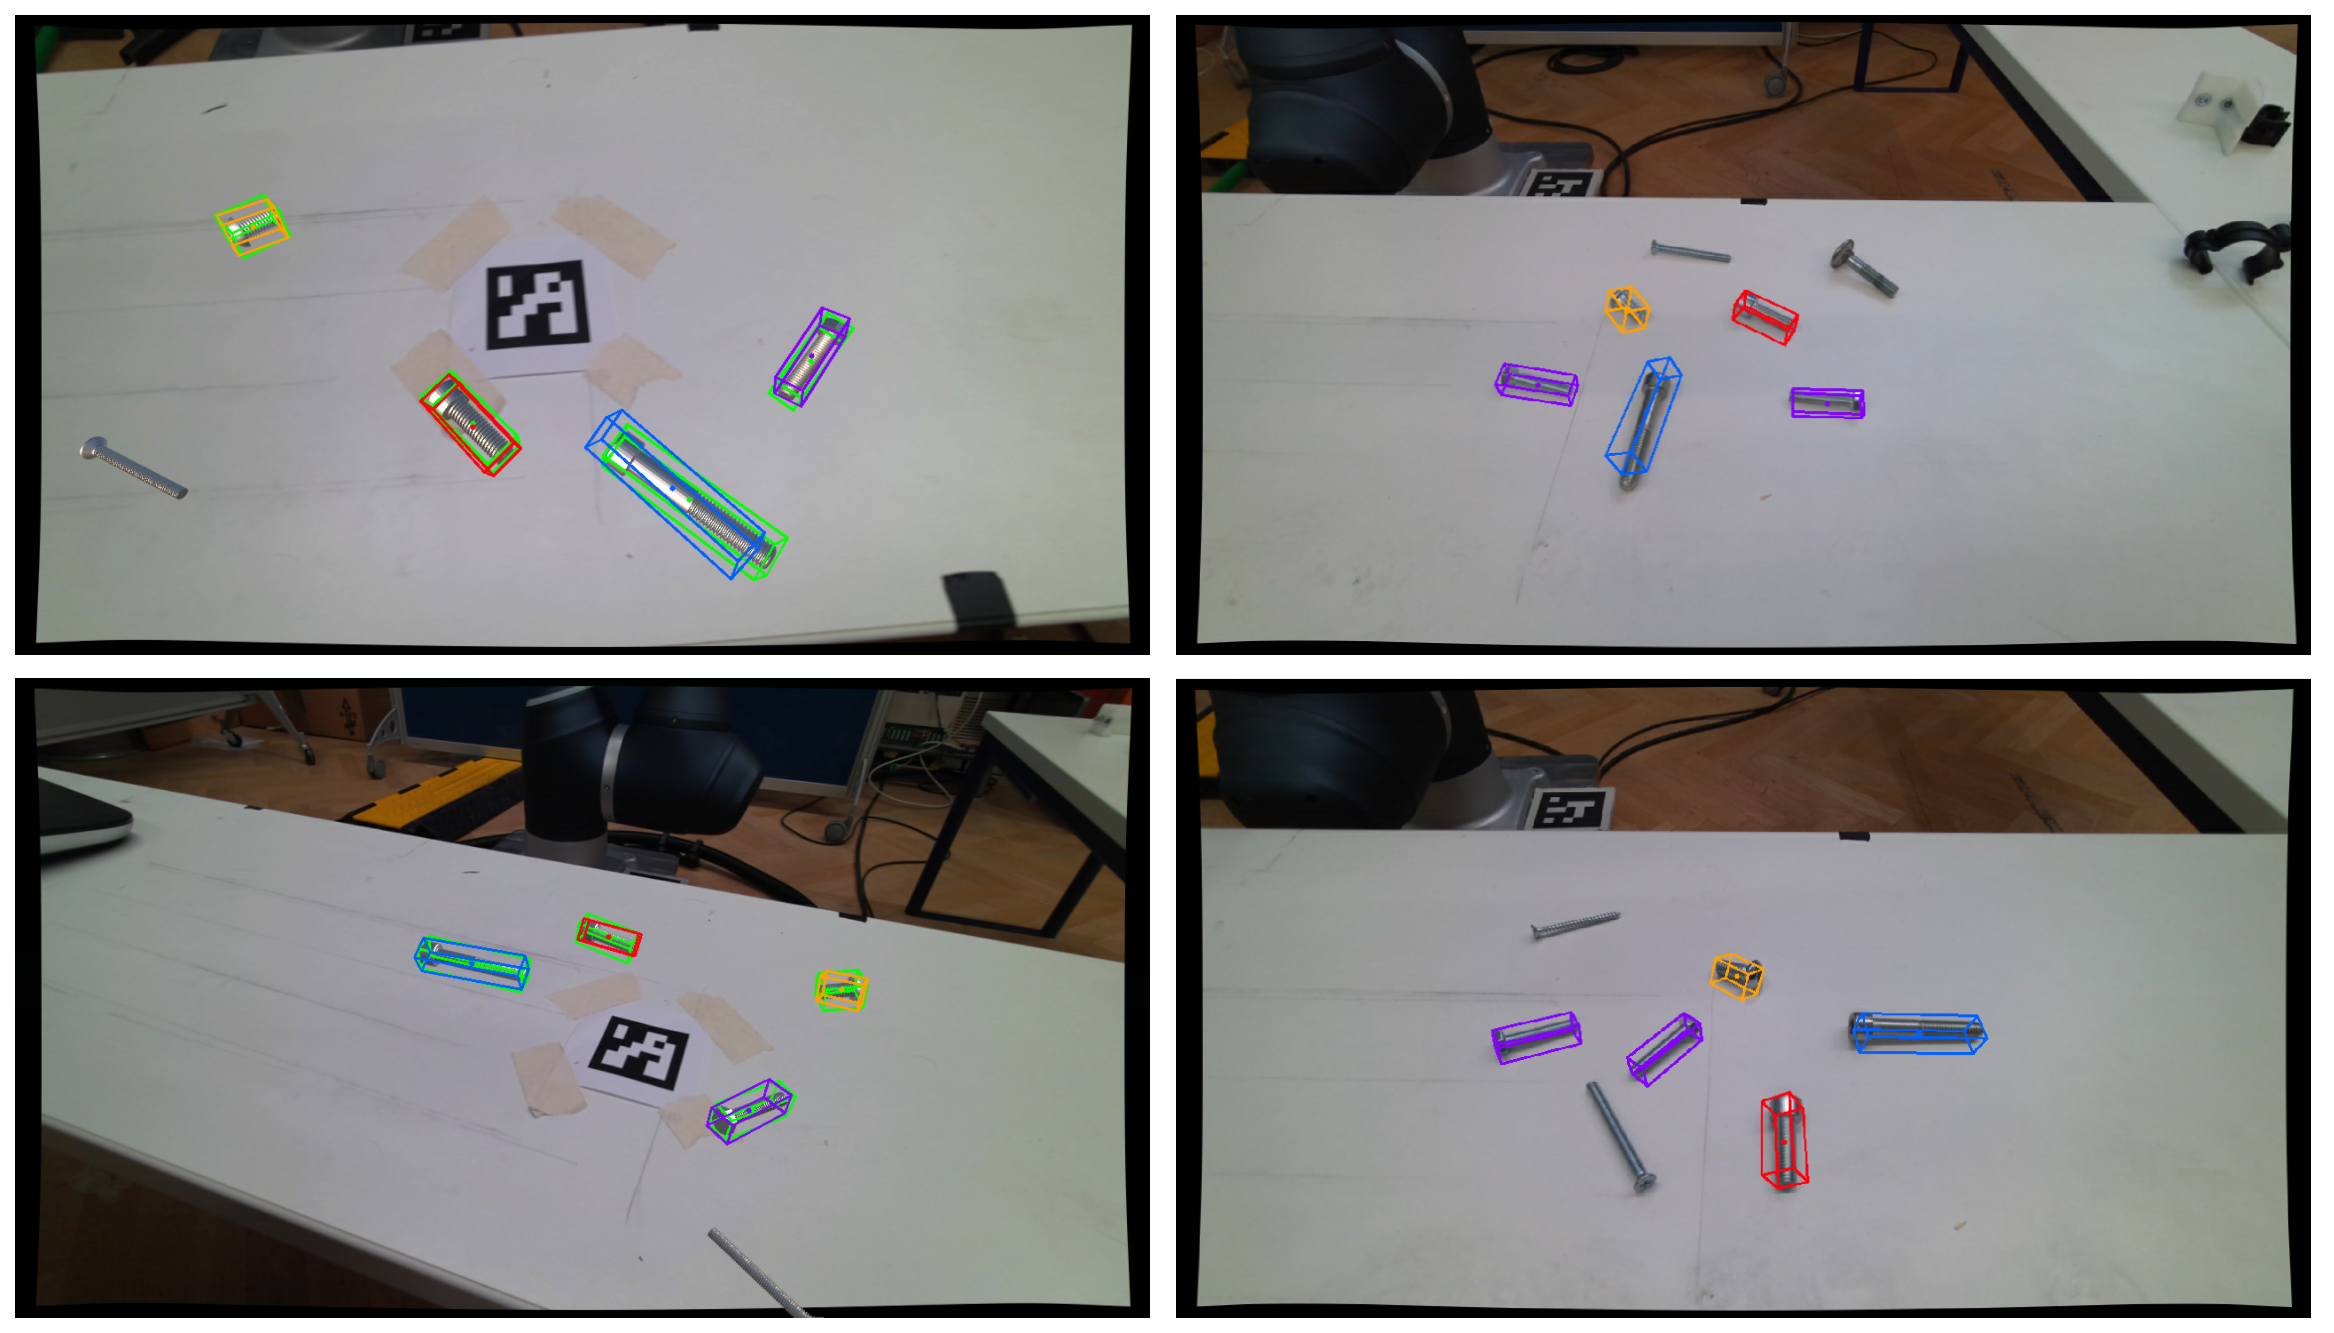
\includegraphics[width=\textwidth]{screwpose_inferencing.png}
    }

    \subfloat[ButtonPose.]{
        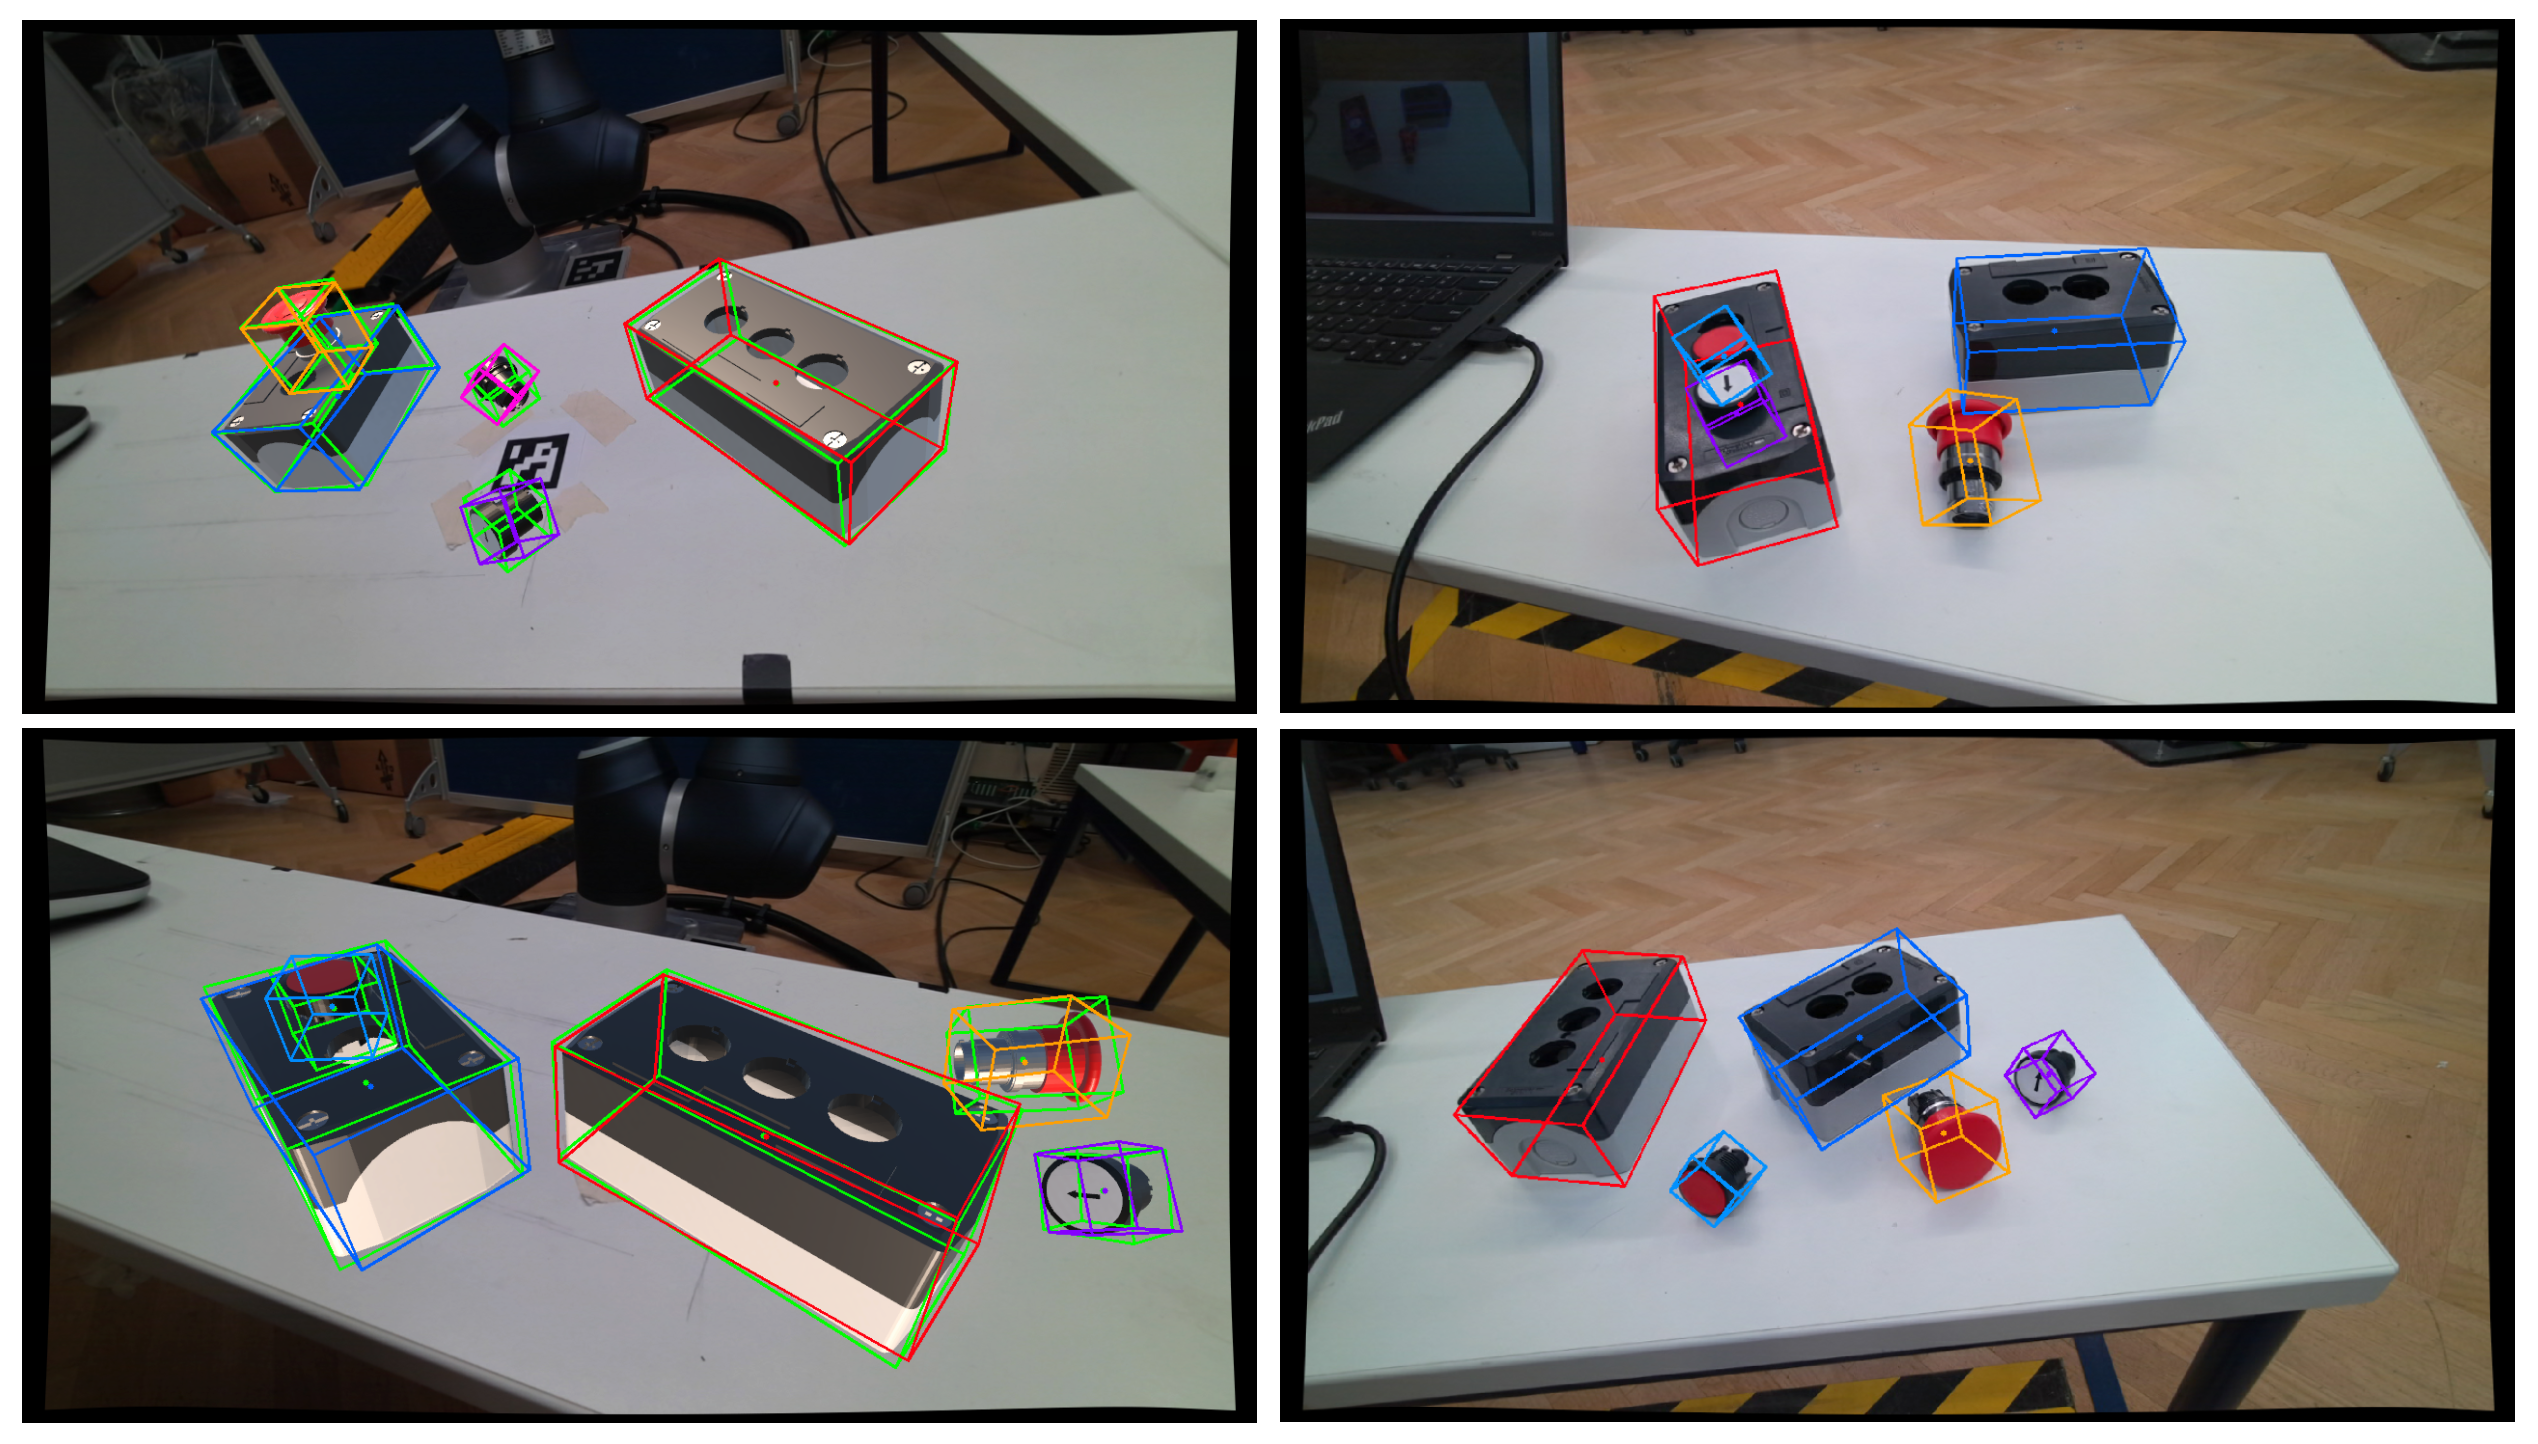
\includegraphics[width=\textwidth]{buttonpose_inferencing.png}
    }

    \caption{Images displaying pose estimations from the network for the ScrewPose and ButtonPose datasets. The left images are part of evaluation and display ground truths with green bounding boxes, the right ones are captures from a real camera in the testing environment.}
    \label{fig:inferencing}
\end{figure}

Finally, training on the ButtonPose dataset resulted in optimal performance for the boards, reaching over 99\% ADD-S and AP for both. The larger safety button also obtained great results, with a 98\% ADD-S, while the other buttons achieved more middling performances, but still better than the Occlusion-LINEMOD benchmark, showing that our approach is valid for more object sets.

The ScrewPose and ButtonPose datasets were also able to generalise to real-life conditions without noticeable losses in performance, as can be observed in figure \ref{fig:inferencing}.

\subsection{Impact of object dimensions and distance}

One noticeable result we observed after training was the impact that physical dimensions have on the final performance of the model for each object. Namely, larger and closer objects have much better performance than smaller and further objects. This is immediately noticeable in the ScrewPose dataset, where the larger M8x50 screw obtained the best results and the M8x16 obtained the worst.

To show how extreme these differences can be, we trained two additional models using new datasets based on the ButtonPose dataset. These two differ solely based on the background images: for the first one the backgrounds were captured from a further distance, while for the second one the backgrounds were captured from close up. For each of these conditions, we captured 50 backgrounds from a variety of positions, and fed them through our dataset generation pipeline. Sample images for these datasets and example positions are shown in figure \ref{fig:near_vs_far}. The close-up dataset (ButtonPose-near hereafter) ended up having an average camera-marker distance of 27.64 cm while the further away dataset (ButtonPose-far hereafter) had an average distance of 49.33 cm.

\begin{figure}[htp]
    \subfloat[ButtonPose-near.]{
        \begin{tabular}{|c||c|c|c|}
            \hline
            Object & AP & AD-S [mm] & ADD-S \\
            \hline \hline
            2-slot & 0.9994 & 2.6850 & 99.94\% \\
            3-slot & 1.0 & 2.8913 & 99.95\% \\
            red button & 0.9663 & 1.3550 & 95.84\% \\
            arrow button & 0.9729 & 1.4384 & 96.47\% \\
            safety button & 1.0 & 1.7229 & 99.84\% \\
            unknown button & 0.9948 & 1.3384 & 98.74\% \\
            \hline \hline
            Average & 0.9889 & 1.9052 & 98.46\% \\
            \hline    
        \end{tabular}
    }

    \subfloat[ButtonPose-far.]{
        \begin{tabular}{|c||c|c|c|}
            \hline
            Object & AP & AD-S [mm] & ADD-S \\
            \hline \hline
            2-slot & 1.0 & 2.9985 & 99.90\% \\
            3-slot & 1.0 & 3.1377 & 99.95\% \\
            red button & 0.5477 & 4.3679 & 29.57\% \\
            arrow button & 0.4902 & 4.4586 & 22.06\% \\
            safety button & 0.9381 & 4.3261 & 79.49\% \\
            unknown button & 0.7489 & 3.7920 & 44.68\% \\
            \hline \hline
            Average & 0.7875 & 3.8468 & 62.61\% \\
            \hline    
        \end{tabular}
    }

    \caption{Evaluation of the Average Precision, Average Symmetric Distance, and ADD-S metrics on the ButtonPose-near and ButtonPose-far datasets after training.}
    \label{fig:near_vs_far_results}
\end{figure}

\begin{figure}[ht]
    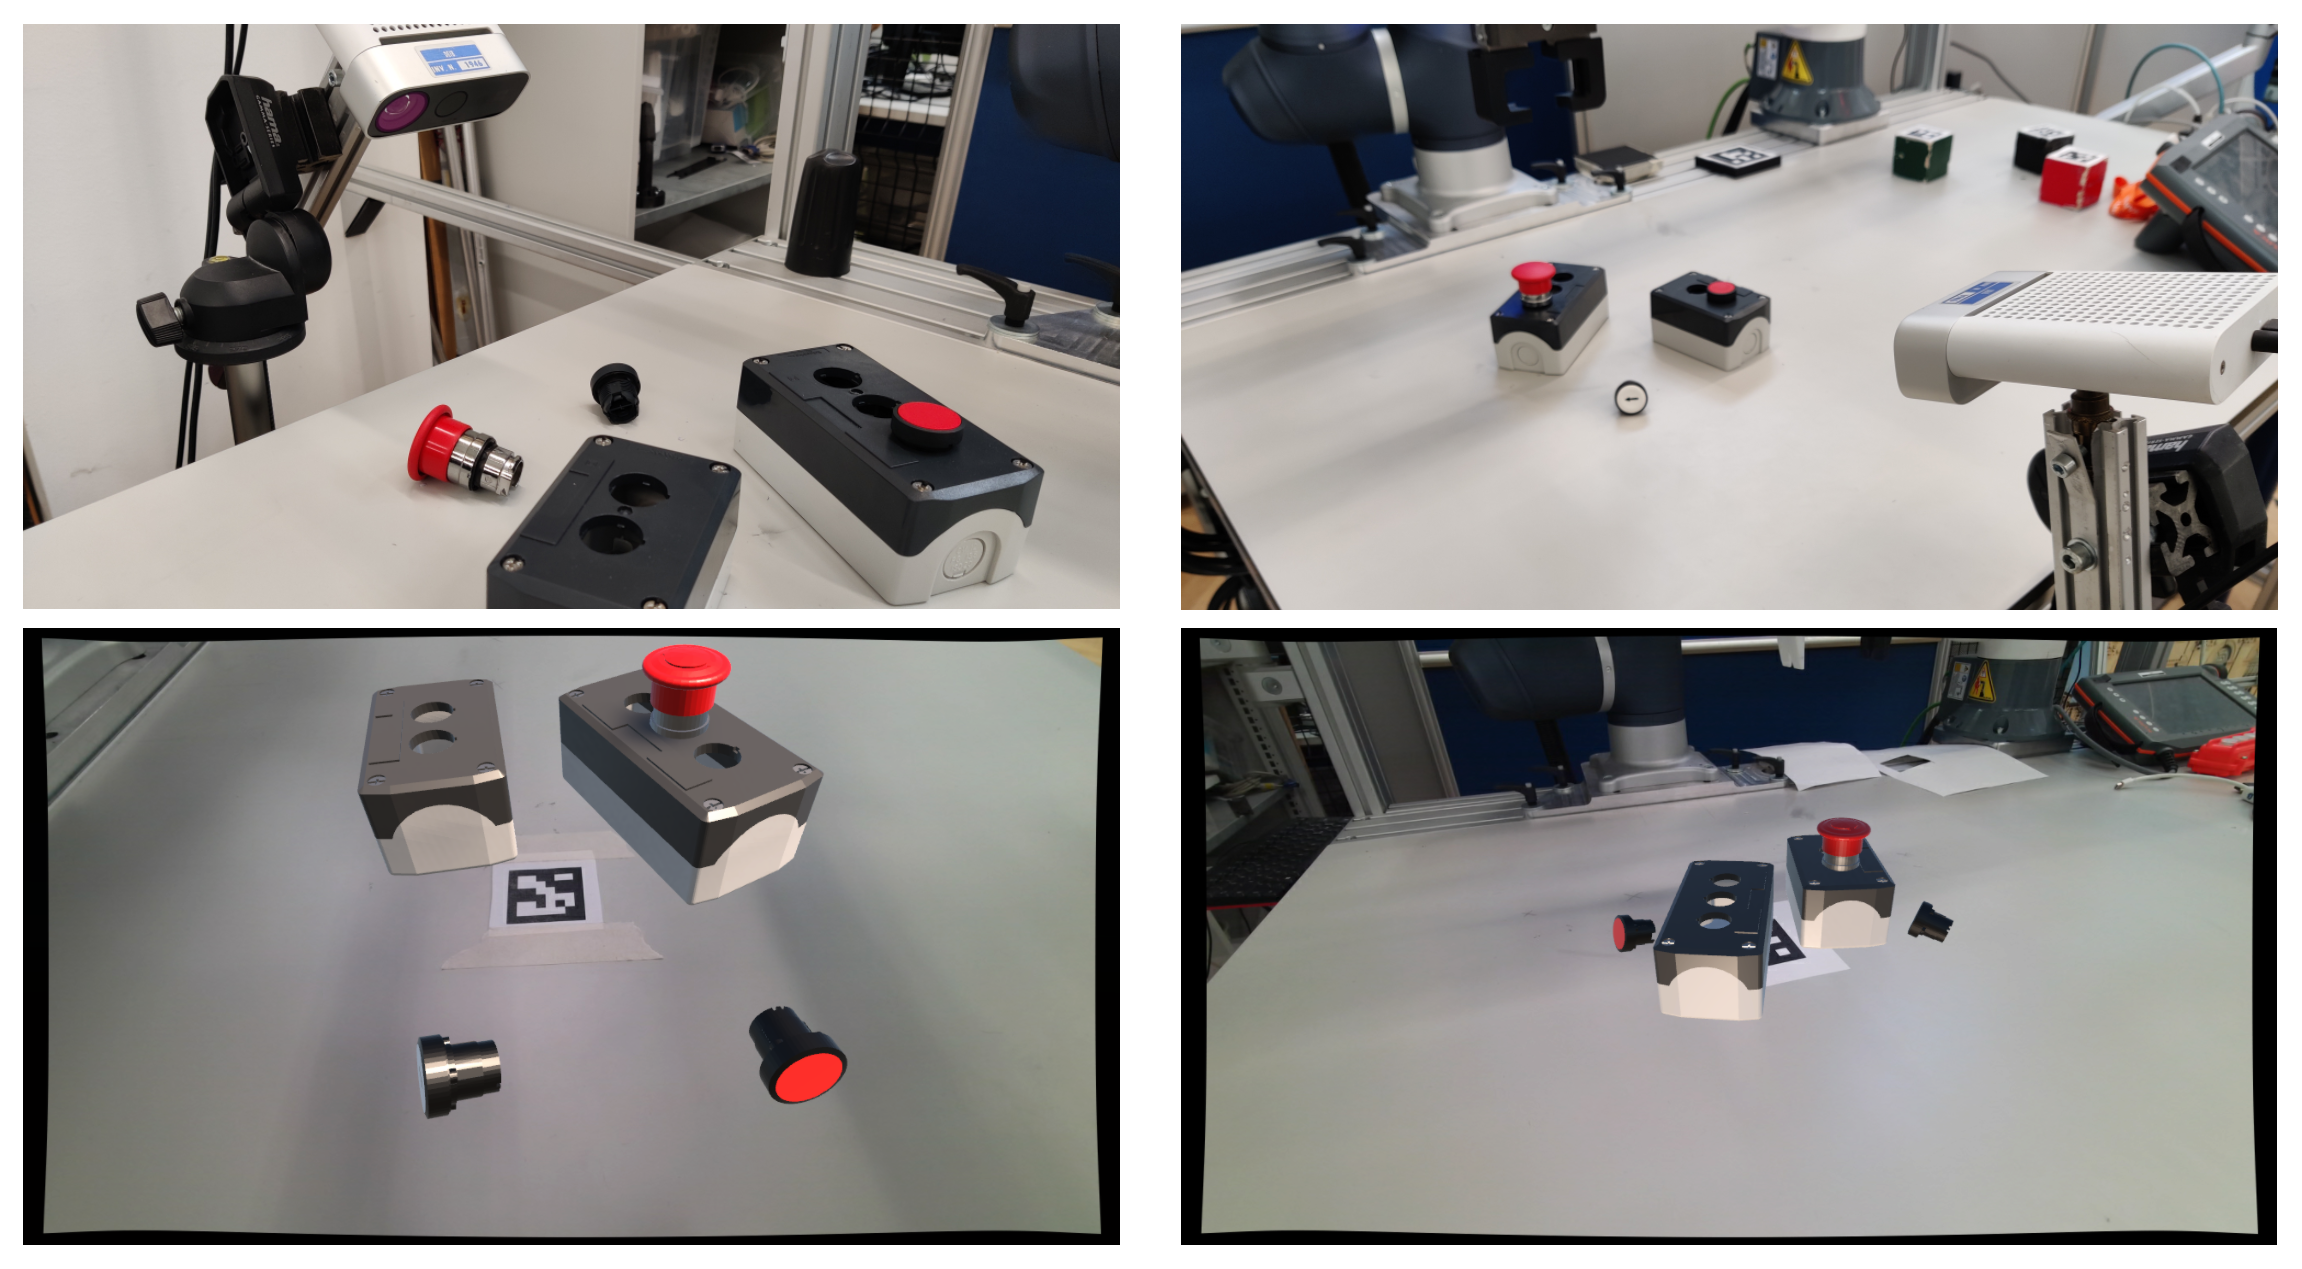
\includegraphics[width=\textwidth]{near_far.png}
    \caption{Photographs of the different capture positions for the ButtonPose-near (left) and ButtonPose-far (right) datasets, with a sample image presented for each.}
    \label{fig:near_vs_far}
\end{figure}

We can then compare the performance of the models trained on the two different datasets, shown in figure \ref{fig:near_vs_far_results}. As can be seen, the -near dataset obtained significantly better results than both the -far dataset and the regular dataset.

We can hypothesize that the reason for such a large gap between the two models lies in the input resolution of the network, which for $\phi = 0$ is set at 512 pixels. This makes it much more difficult for the network to make out fine details at a distance; in particular it would struggle to distinguish between the arrow button and the red button, since their faces would appear similar. This issue could therefore probably be alleviated by using higher values of $\phi$.

\subsection{False Positive Issues}
\label{false_positives_issue}

\begin{figure}[ht]
    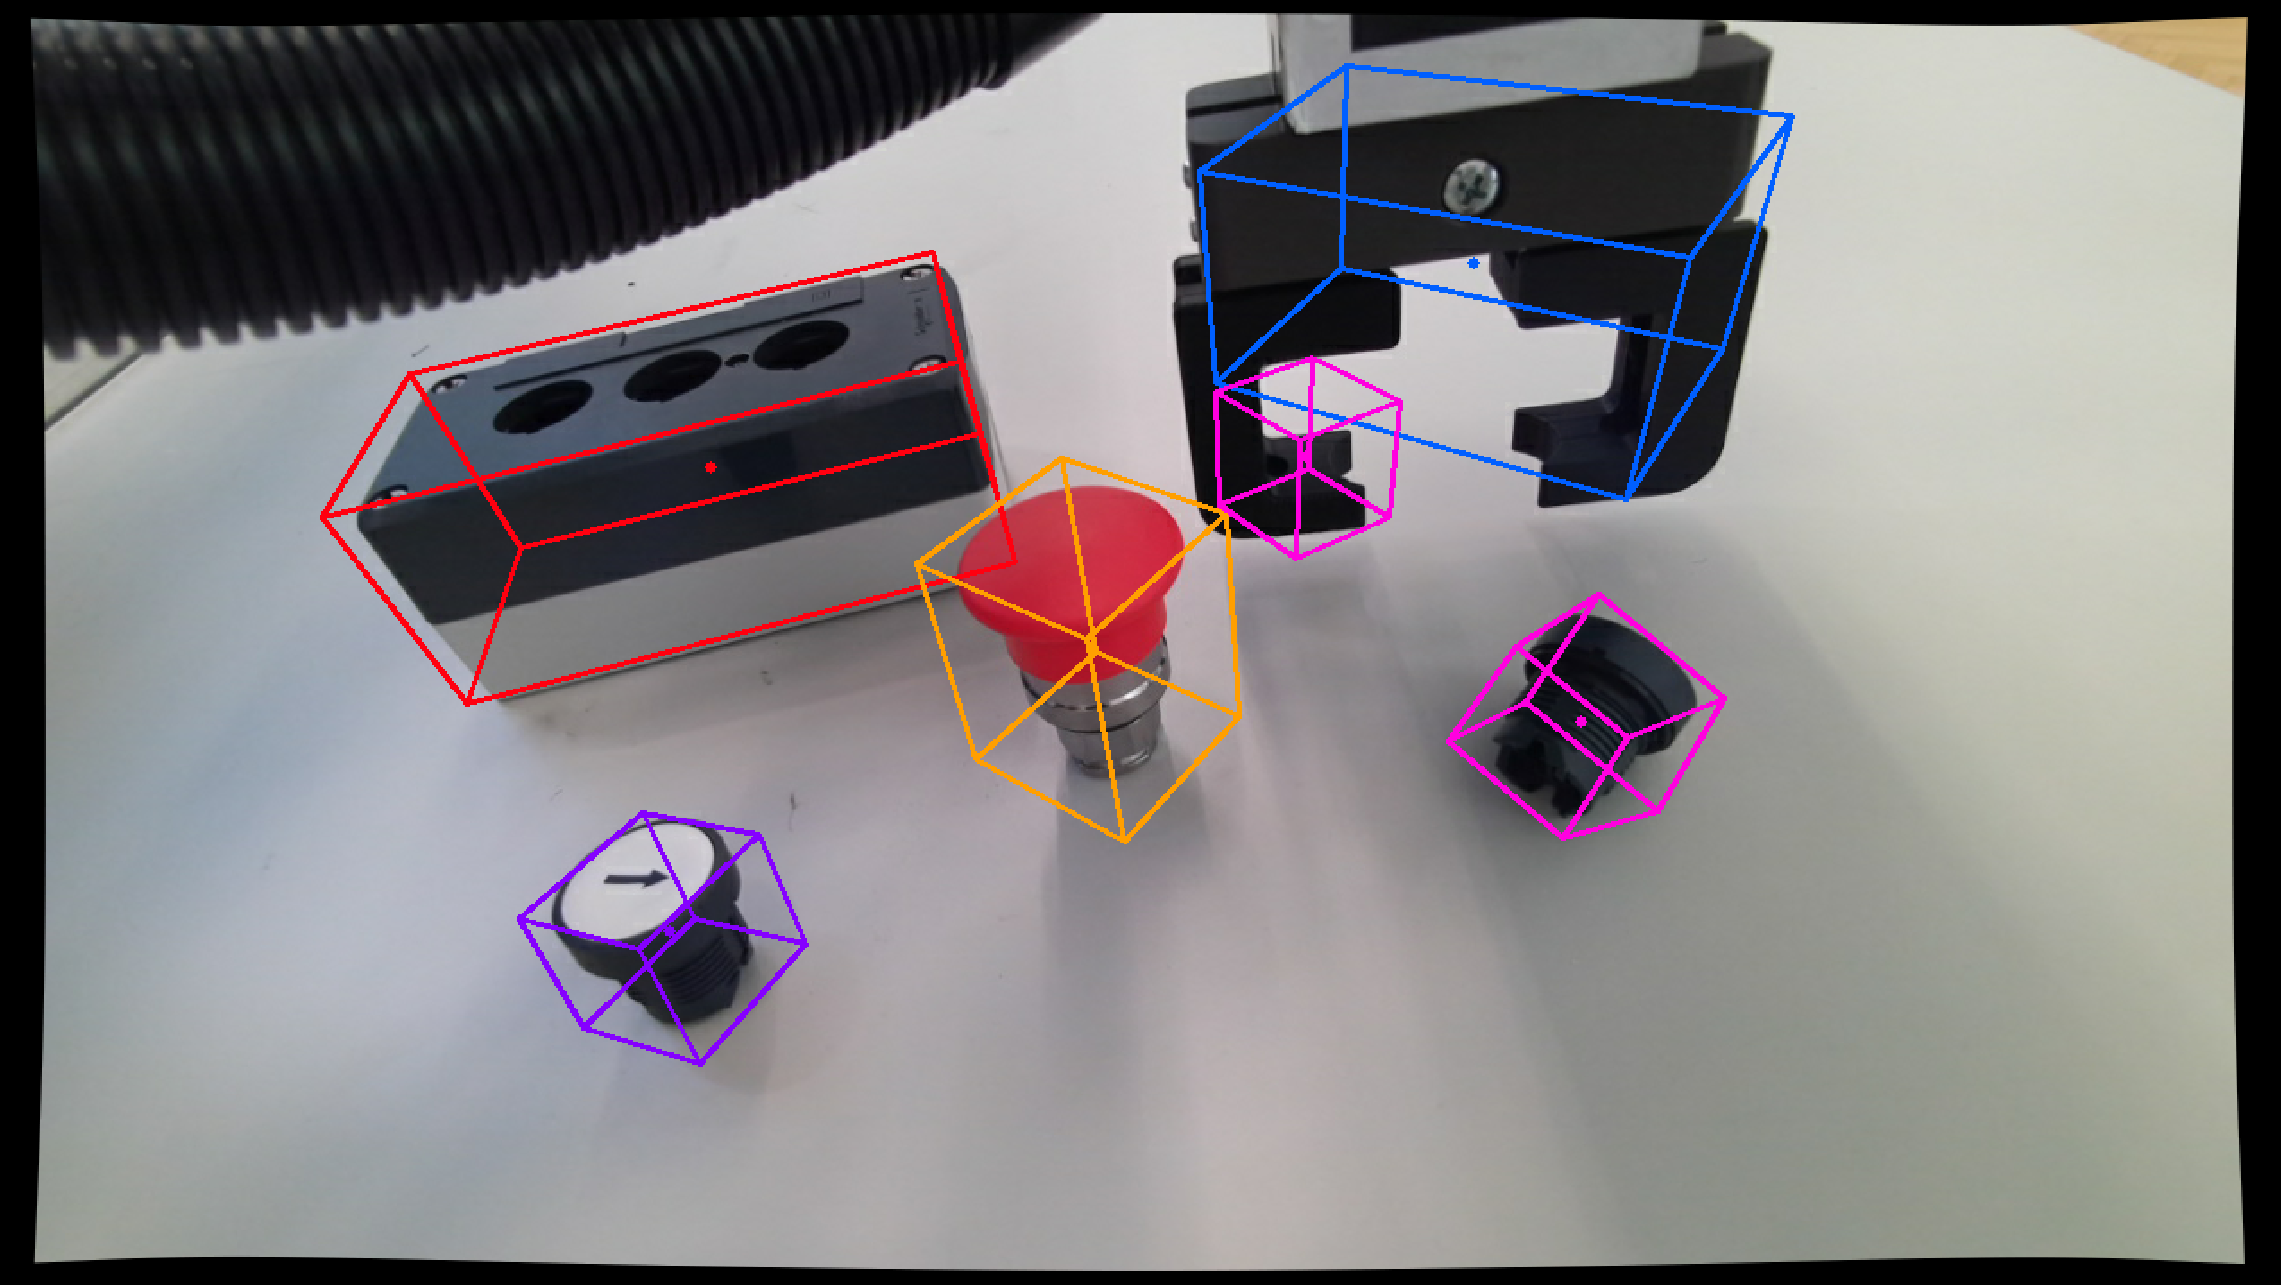
\includegraphics[width=0.7\textwidth]{false_positives.png}
    \caption{An example of how introducing untrained objects results in false positives.}
    \label{false_positives}
\end{figure}

A noticeable issue we encountered when testing our models in real world conditions was the difficulties they expressed in dealing with objects that are not present in the original dataset. In almost all cases, introduction of a never-before-seen object results in multiple false positives, as shown in figure \ref{false_positives}. This is because the model is not trained to "ignore" these objects, and thus attempts to classify them according to what it effectively "knows".

There are ways to approach and mitigate this issue. For example, if there is a high probability that a certain object that should not be tracked by the model will appear frequently in the scene, one could include that object within the dataset generation method without labelling it. In this manner, since the object would appear with a certain frequency during training, eventual false positives resulting from its presence would be recognized as such, and the model's behavior corrected.

We tested this method with the ScrewPose dataset: since all of its objects have a similar shape, a model trained on ScrewPose would tend to categorize any long and thin object as a screw, making it especially susceptible to false positives. However, introducing a "dummy" screw into most images, without labelling it as a dataset object, led to the model subsequently ignoring its appearance in most scenes. It was also able to generalise this behavior to a certain extent, ignoring other never-before-seen screws when they were introduced into the scene (see figure \ref{fig:inferencing}). Therefore in a case such as the one represented in figure \ref{false_positives}, if we were certain of the appearance of the gripper in many scenes, it would be worthwile to include its 3D model in some training images, so that the network could effectively learn to ignore it.

We hypothesize that by including a general enough set of "dummy" items in the training images, the model could then generalize this behavior to a wider variety of previously unseen objects. However, due to the nature of black-box methods, more research is necessary to verify whether this is feasible.

\section{Semantic Meaning Extraction Results}

In this section we will evaluate the performance of our semantic meaning extraction method. The precision-recall curves in figure \ref{fig:precisionrecall} were computed using the methodology described in section \ref{semantics_method_section} on the ButtonPose and ButtonPose-near datasets. The optimal thresholds and F1 scores are laid out in figure \ref{fig:optimal_F1}.

\begin{figure}[htp]
    \centering
    \subfloat[ButtonPose]{
        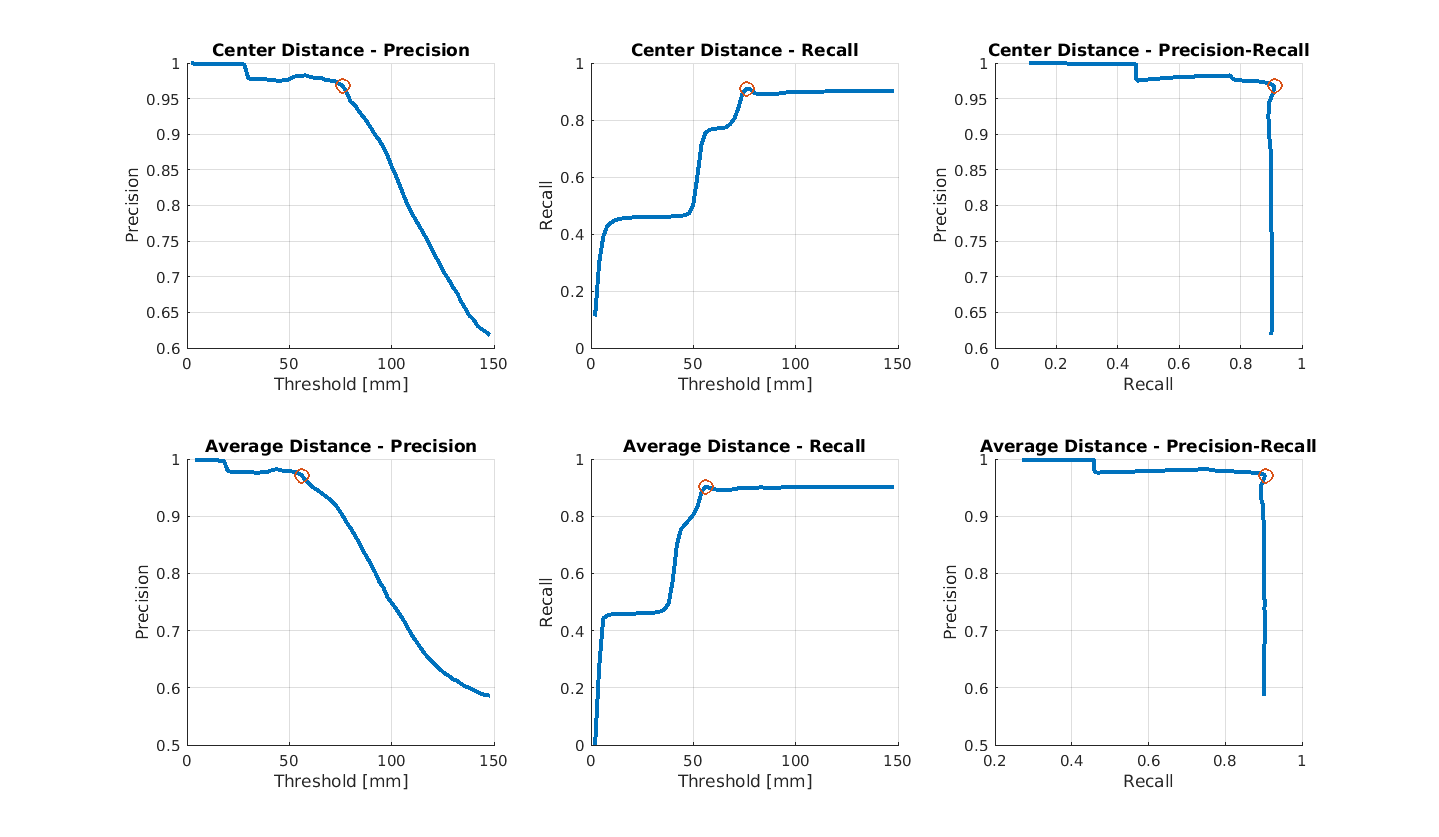
\includegraphics[width=\textwidth]{precision-recall.png}
    }

    \subfloat[ButtonPose-near]{
        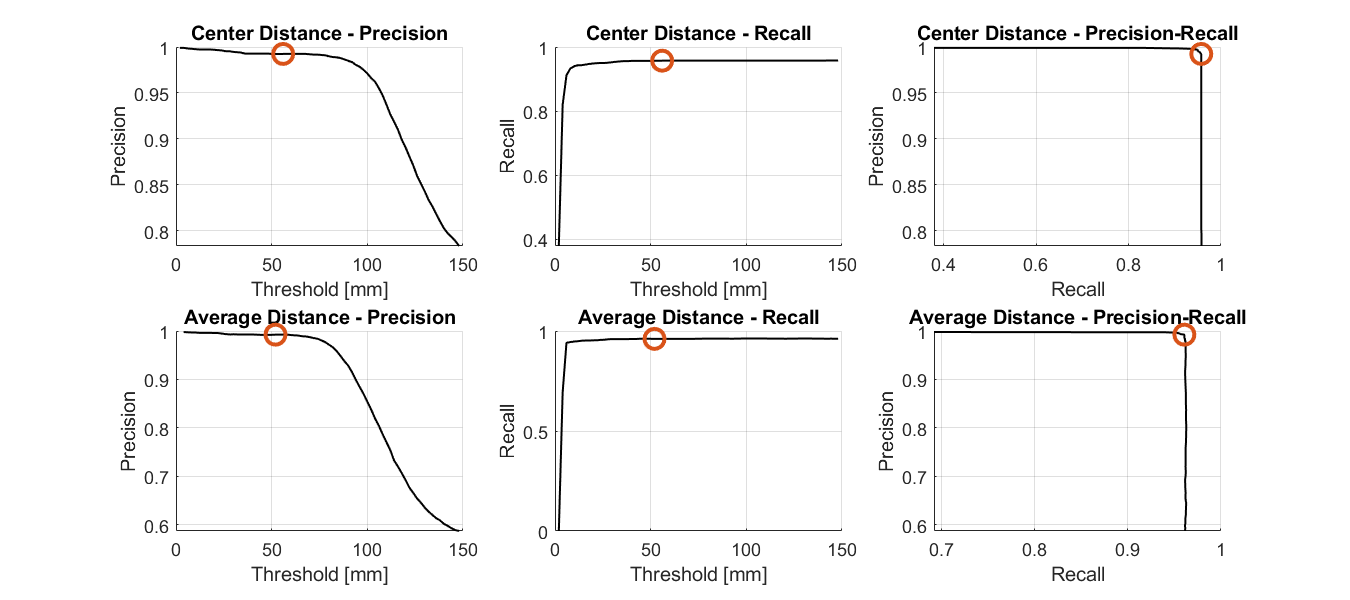
\includegraphics[width=\textwidth]{precision-recall_near.png}
    }
    
    \caption{Precision and recall for both distance metrics on the ButtonPose and ButtonPose-near datasets. The point with the best F1 score is highlighted with a red circle in both cases.}
    \label{fig:precisionrecall}
\end{figure}

\begin{figure}
    \subfloat[ButtonPose]{
        \begin{tabular}{|c||c|c|}
            \hline
            Metric & F1 & Threshold \\
            \hline \hline
            AD & 0.9369 & 56mm \\
            CC & 0.9255 & 78mm \\
            \hline
        \end{tabular}
    }
    \quad
    \subfloat[ButtonPose-near]{
        \begin{tabular}{|c||c|c|}
            \hline
            Metric & F1 & Threshold \\
            \hline \hline
            AD & 0.9763 & 52mm \\
            CC & 0.9746 & 56mm \\
            \hline
        \end{tabular}
    }
    
    \caption{Optimal F1 scores and thresholds for both the Average Distance (AD) and Center-to-Center (CC) metrics on the ButtonPose and ButtonPose-near datasets.}
    \label{fig:optimal_F1}
\end{figure}

Overall our method shows promising results, with precision-recall curves that are similar to the ideal, and high F1 scores.

We observe that our application obtained no great advantage in using Average Distance over Center-to-Center distance. Given the additional complexity and computation time, the increase in performance is not significant: for reference, computing the values for figure \ref{fig:precisionrecall} took 23.67 seconds using Center-to-Center, and 2650.34 seconds using Average Distance, making the second approximately 112 times slower.

We also obtained high values for the optimal \emph{distance thresholds}, above 5 cm in all testing conditions. We take this to mean that our method applies the threshold to determine whether a button is in a slot at all, while the slot itself is selected using the conflict resolution strategy previously described.

We hypothesize that the reason for this behavior lies in the dataset generation algorithm: by stating that the buttons can exclusively be either inside a slot or placed on the surface, we are in fact considering an ideal situation where a theoretical manipulator does not commit any errors in picking up and inserting the buttons. If failed attempts were considered in the dataset, it is likely that the optimal threshold would be lower, and the Average Distance method, being more sensible to situations with different rotations, would likely give better results than Center-to-Center.

Finally, the value of the threshold is also influenced by the probability distribution used for generating the poses for the button dataset, which in our case being a uniform distribution, resulted in a more spread-out placement, thus a higher optimal threshold. This is further compounded by the brute-force collision avoidance strategy implemented within the placement algorithm: if a placement attempt would generate an intersection with an already placed object, the placement is simply re-attempted from scratch. This naturally results in less conditions where dataset objects are in close proximity, and therefore in a higher threshold.

\section{Real-World Application Results}

As previously described in section \ref{semantics_method_section}, we tested the performance of our vision method in a real-world application where the robot had to pick up a button from the ButtonPose dataset and insert it into a slot on one of the button boards. while relying solely on RGB images.

\begin{table}
    \begin{center}
        \begin{tabular}{|c|cc|}
            \hline
            Button Type & Small & Large \\
            \hline
            Total Attempts & 10 & 10 \\
            \hline
            Successful Pick-Ups & 7 & 10 \\
            \hline
            Successful Insertions & 5 & 7 \\
            \hline

        \end{tabular}
    \end{center}
\end{table}

In our testing, the robot was able to pick up the smaller buttons seven times out of ten, while it was able to pick up the larger button in all test cases. Out of the times it was able to pick up a button, the following insertion was performed correctly in 72\% of cases.

The main issue encountered during testing was the prevalence of small errors in the rotation of the gripper relative to the button. These errors are usually in the neighborhood of $\pm5\degree$, but they are noticeable and can lead to mistakes, as the button may be gripped in an awkward manner.

\begin{figure}[ht]
    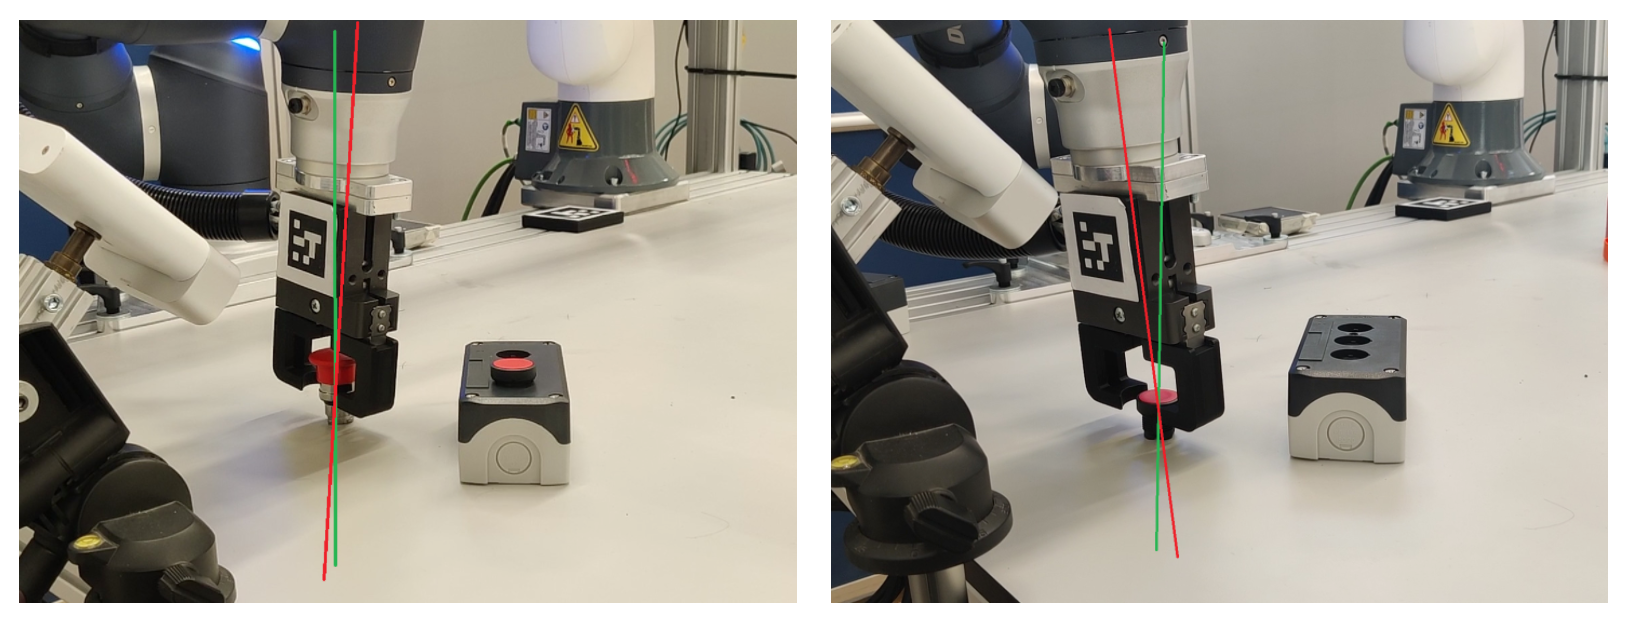
\includegraphics[width=\textwidth]{roboterrors.png}
    \caption{Examples of small rotation errors when attempting to pick up a button with the robotic arm. The green line indicates the button's central axis, while the red line is the robot's.}
\end{figure}

Positioning relative to the boards was instead very accurate, and errors is the insertion phase were mostly due to mistakes in grasping the necessary buttons.

Overall the robot performed much better when dealing with the larger buttons and boards than when dealing with the smaller buttons, making its reliability very dependant on the accuracy of the pose estimation network. The network proved to be relatively accurate regarding the 3D position of objects, but often not as accurate regarding their rotation, leading to small mistakes that overall may have negative effects on tasks requiring high precision.

\chapter{Conclusions}

In the field of robotics, and automation in general, the interactions between the autonomous system, or robot, and the environment, are of fundamental importance. Perception in particular requires the system to have a certain number of sensors that provide it with data on the environment, which it then processes to obtain the information necessary to perform its purposed task.

RGB Color cameras, while being relatively cheap and easily sourceable sensors, introduce a series of difficulties and complications that limit their applicability in real-time control applications. However, neural networks, and convolutional neural networks in particular, are perfectly suited to cover these issues.

Due to this,  rapid developments in the fields of object identification and pose estimation techniques have occurred and, there has been an increased interest in applying these techniques to tasks for industrial and collaborative robotics. However, due to the challenges introduced by machine learning approaches, the viability and performance of these methods in a real world application remained to be seen.

To tackle these issues, we began by developing a dataset generation algorithm to simplify the data acquisition phase. While unfortunately a more general approach involving fully rendering the training images failed to produce satisfactory results, a more specific technique involving realistically placing objects inside of a photograph proved to be effective. These generated datasets resulted in excellent performance, that did not decline in a noticeable manner when tested in a real-world environment.

We then developed a method to extract the high-level semantic state of a scene, starting from the results of an inference performed by the trained pose estimation network. We applied a simple thresholding technique, while devising methods to manage various issues, such as the occlusion of identifying features and conflicts resulting from higher values of the distance threshold. The performance of the resulting method was excellent, though it is highly dependant on the performance of the underlying network.

Finally, we applied the complete network and semantics method to a real-world application. By "teaching" a robotic manipulator how to perform basic actions using kinesthetic demonstrations, the overall system was able to plan and complete simple assembly tasks. However, these experiments highlighted how the system struggled with smaller objects, with consistent small errors in rotation estimations that detracted from its overall performance.

In conclusion, object detection and pose estimation approaches have remarkable performance in robotics applications, but may be insufficient in tasks that require high precision and reliability, or tasks involving small objects, or objects that are difficult to identify in other ways.

Furthermore, the black-box nature of neural networks means that the performance of our own approach and datasets may be compromised when applied to a radically different environment than the one used for dataset generation and training, thus requiring a new dataset and training for the new environment. This is the main disadvantage of our approach, that it is specific on one environment.

In the future, it could be possible to progress and improve upon our work. We considered for example:
\begin{itemize}
    \item Comparing the performance of a network trained on one of our generated datasets with a network trained on real-world labelled data, with the same objects and in the same environment.
    \item Verifying the possibility of avoiding false positives with the model by training it to ignore objects.
    \item When generating a dataset, verifying whether including multiple different environments in the background improves generalisiation, or whether this is unnecessary.
    \item If future pose estimation approaches increase performance in a significant manner, verifying whether they obtain the accuracy required for high precision robotics applications.
\end{itemize}

% LIST OF FIGURES
\listoffigures
\addcontentsline{toc}{chapter}{List of Figures}

% LIST OF TABLES
\listoftables
\addcontentsline{toc}{chapter}{List of Tables}

\bibliography{bibliography}
\addcontentsline{toc}{chapter}{Bibliography}

\end{document}
